This chapter introduces the background knowledge used in this project's development. This chapter includes two main sections: Multimodal Models and Visual Reasoning Datasets. \cref{sec:multimodal_models} explains the types of models that are related to this work. \cref{sec:visual_reasoning_datasets} includes synthetic and natural visual reasoning datasets and the datasets that we chose for this work.

\section{Multimodal Models} \label{sec:multimodal_models}

Multimodal models are trained jointly on text and image pairs. This is different from language models, which are only trained with text and vision models which only use images. The aim of VLMs is to ground LMs with visual concepts.

This section explains the types of models that are related to this work, Multimodal Transformers, Multimodal RNNs and Diffusion Models. \cref{sec:multimodal_transformers} includes descriptions of the following \textbf{multimodal transformers}: OFA \cite{wang2022unifying}, BLIP \cite{li2022blip}, CLIP \cite{radford2021clip}, OpenCLIP \cite{ilharco_gabriel_2021_5143773}, FLAVA \cite{singh2022flava}, LXMERT \cite{tan2020lxmert}, UniT \cite{hu2021unit}, UNITER \cite{chen2020uniter}, VILLA \cite{gan2020villa}, VinVL \cite{zhang2021vinvl}, ViLT \cite{kim2021vilt}, VisualBERT \cite{li2019visualbert} and ViLBERT \cite{lu2019vilbert}. \cref{sec:multimodal_transformers} explains two types of \textbf{multimodal RNN} models: VSE++ \cite{faghri2018vse} and VSRN \cite{li2019vsrn}. \cref{sec:diffusion_models} introduces \textbf{diffusion models} and explains Stable Diffusion \cite{rombach2021highresolution}, the diffusion model that we use in this work.

\paragraph{Overview.}
\cref{tab:model-types} provides a high-level overview of the Transformer and RNN models that are described in the next sections. This overview includes pretraining datasets, architecture, and attention mechanisms between the modalities. We omit datasets that were only used to train backbones. We exclude the language embedding from this table as every model uses a pretrained BERT tokenizer, except CLIP, VSE++, and VSRN. The pretraining datasets include COCO \cite{lin2014microsoft}, Visual Genome (VG) \cite{krishna2016visual}, Conceptual Captions (CC) \cite{sharma2018conceptual}, SBU Captions \cite{ordonez2011im2text}, Flickr30k \cite{young2014image}, VQA 2.0 \cite{goyal2017making}, VCR \cite{zellers2019recognition}, NLVR2 \cite{suhr2017corpus}, SNLI-VE \cite{xie2018visual}, QNLI \cite{rajpurkar2016squad}, MLNI-mm \cite{williams2017broad}, QQP \cite{QQPDataset}, Localized Narratives (LN) \cite{pont-tuset2020localized-narratives}, Wikipedia Image Text (WIT) \cite{srinivasan2021wit}, Conceptual Captions 12M (CC 12M) \cite{changpinyo2021conceptual12m}, Red Caps (RC) \cite{desai2021redcaps}, YFCC100M \cite{thomee2016yfcc100m}, SST-2 \cite{Socher2013RecursiveDM}, LAION-400M \cite{schuhmann2021laion} and LAION-2B \cite{schuhmann2022laionb}. CLIP uses their own dataset for pretraining.

\begin{table}[ht]
    \centering
    \small
    \begin{adjustbox}{max width=\textwidth}
    \begin{tabular}{l|lr|l|l}
    \toprule
    Model & Datasets & \# Images, Captions & Architecture & Attention \\\midrule
    VinVL \cite{zhang2021vinvl}  & VQA, GQA, VG-QA, COCO, Flickr30k, CC, SBU & 1.89, 4.87 & single-stream & merged \\
    UNITER \cite{chen2020uniter}  & COCO, VG, CC, SBU & 4.20, 9.58 & single-stream  &  merged \\
    ViLLA \cite{gan2020villa} & COCO, VG, CC, SBU  & 4.20, 9.58 & single-stream  &  merged \\
    VisualBERT \cite{li2019visualbert}& COCO, NVLR2 & 0.30, 0.52  & single-stream  & merged \\
    ViLT \cite{kim2021vilt}  & COCO, VG, SBU, CC & 4.10, 9.85 & single-stream  & merged \\
    LXMERT \cite{tan2020lxmert}  & COCO, VG & 0.18, 9.18 & dual-stream & modality-specific, co-attn, merged \\
    ViLBERT \cite{lu2019vilbert}  & CC & 3.30, 3.30 & dual-stream  & modality-specific, co-attn, merged \\
    UniT \cite{hu2021unit} & COCO, VG, VQAv2, SNLI-VE QNLI, MNLI-mm, QQP, SST-2 & 0.69, 1.91 & dual-stream & modality-specific, merged\\
    FLAVA $_{ITM}$ \cite{singh2022flava}  & COCO, SBU, LN, CC, VG, WIT, CC 12M, RC, YFCC100M & 70.00, 70.00 & dual-stream & modality-specific, merged \\
    FLAVA $_{ITC}$ \cite{singh2022flava}  & COCO, SBU, LN, CC, VG, WIT, CC 12M, RC, YFCC100M & 70.00, 70.00 & dual-stream & modality-specific \\
    CLIP \cite{radford2021clip}  & $-$ & 400.00, 400.00 & dual-stream & modality-specific \\
    OpenCLIP \cite{ilharco_gabriel_2021_5143773}  & LAION-2B & 2320.00, 2320.00 & dual-stream & modality-specific \\
    OFA \cite{wang2022unifying} &  CC 12M, CC 3M, SBU, COCO, VG-Cap  &  20.00, 20.00 &   single-stream & modality-specific, merged \\
    BLIP$_{ITM}$ 14M \cite{li2022blip} &  COCO, VG, SBU, CC, CC 12M  &  14.00, 15.00 &   dual-stream & modality-specific, merged \\
    BLIP$_{ITC}$ 14M \cite{li2022blip} &  COCO, VG, SBU, CC, CC 12M & 14.00, 15.00 &   dual-stream &         modality-specific \\
    BLIP$_{ITM}$ 129M \cite{li2022blip} & COCO, VG, SBU, CC, CC 12M, LAION-400M & 129.00,   130.00 &   dual-stream & modality-specific, merged \\
    BLIP$_{ITC}$ 129M \cite{li2022blip} & COCO, VG, SBU, CC, CC 12M, LAION-400M & 129.00,   130.00 &   dual-stream &         modality-specific \\
    VSE++ $_{COCO}$ \cite{faghri2018vse} & COCO & 0.11, 0.57 & dual-stream & $-$\\
    VSE++ $_{Flickr30k}$ \cite{faghri2018vse} & Flickr30k & 0.03, 0.16 & dual-stream & $-$\\
    VSRN $_{COCO}$ \cite{li2019vsrn}  & COCO & 0.11, 0.57 & dual-stream & $-$\\
    VSRN $_{Flickr30k}$ \cite{li2019vsrn} & Flickr30k & 0.03, 0.16 & dual-stream & $-$\\
    \bottomrule
    \end{tabular}
    \end{adjustbox}
    \caption{A high-level overview of the differences between the models by the pretraining datasets, architecture, and attention mechanisms between the modalities.}
    \label{tab:model-types}
\end{table}

\subsection{Multimodal Transformers} \label{sec:multimodal_transformers}

Multimodal transformers are state-of-the-art in many vision-language tasks, and that includes spatial reasoning. Most of the models tested in Winoground \cite{thrush2022winoground} and VSR \cite{liu2022visual} are multimodal transformers. Those transformers differ in embedding, architecture, pretraining objectives and cross-modal attention. First, we provide some examples of different types of transformers. Then, we describe every model that was used in previous and current experiments.

\textbf{Embedding.} Most models use a pretrained BERT tokenizer for text encoding. For image embedding, there are more different options. Some models use Faster R-CNN~\cite{ren2015faster} to extract region features from images: VisualBERT, ViLBERT, LXMERT, UNITER, ViLLA \cite{li2019visualbert,lu2019vilbert,tan2020lxmert,chen2020uniter,gan2020villa}. Another common approach is to use Vision Transformer (ViT) \cite{dosovitskiy2020imageworth}, which is used by CLIP, FLAVA, and ViLT \cite{radford2021clip, singh2022flava, kim2021vilt}.

\textbf{Architecture.} Depending on their architecture, they can mainly be classified into two types: single-stream and dual-stream transformers. On the one hand, in \textbf{single-stream} transformers the image and text embeddings are concatenated and then jointly encoded. For instance, the following transformers are single-stream: UNITER, VILLA, VinVL, ViLT and VisualBERT. \cite{chen2020uniter, gan2020villa, zhang2021vinvl, kim2021vilt, li2019visualbert}. On the other hand, \textbf{dual-stream} transformers have two separate modality-specific encoders with optional cross-modality fusion. Some examples include: CLIP, FLAVA, UniT, LXMERT and ViLBERT \cite{radford2021clip, singh2022flava, hu2021unit, tan2020lxmert, lu2019vilbert}.

\textbf{Cross-Modal Attention.} There are different types of multimodal attention as presented in \cite{hendricks2021decoupling}. In \textbf{modality-specific attention}, the language and visual input attend to their modality. Every dual-stream transformer that we mentioned uses this type of attention. In \textbf{merged attention}, the language and visual input attend to both themselves and the other modality. All single-stream models use merged attention, and some dual-stream transformers use it too. In \textbf{co-attention}, the language and visual input only attend to the other modality input. For example, dual-stream models LXMERT and ViLBERT use co-attention.

\textbf{Pretraining Objectives.} Vision-language transformers use a different pretraining objectives including \textbf{masked language modeling} (MLM), image-conditioned \textbf{language modeling} (LM), \textbf{image-text contrastive} learning (ITC), \textbf{image-text matching} (ITM). For Winoground, we are mainly interested in models that are trained with ITC or ITM objectives. For example, BLIP \cite{li2022blip} is jointly pre-trained with three vision-language objectives: ITC, ITM and LM.

\paragraph{LXMERT.} LXMERT \cite{tan2020lxmert} consists of  three transformer encoders: object relationship encoder, a language encoder, and a cross-modality encoder (see \cref{fig:lxmert}). The images are represented as a sequence of objects, whereas each sentence is a sequence of words. It combines self-attention and cross-attention layers to generate language, image, and cross-modality representations. The model is pre-trained with five pre-training tasks: masked language modelling, masked object prediction, cross-modality matching, and image question answering.

\begin{figure}[ht]
    \centering
    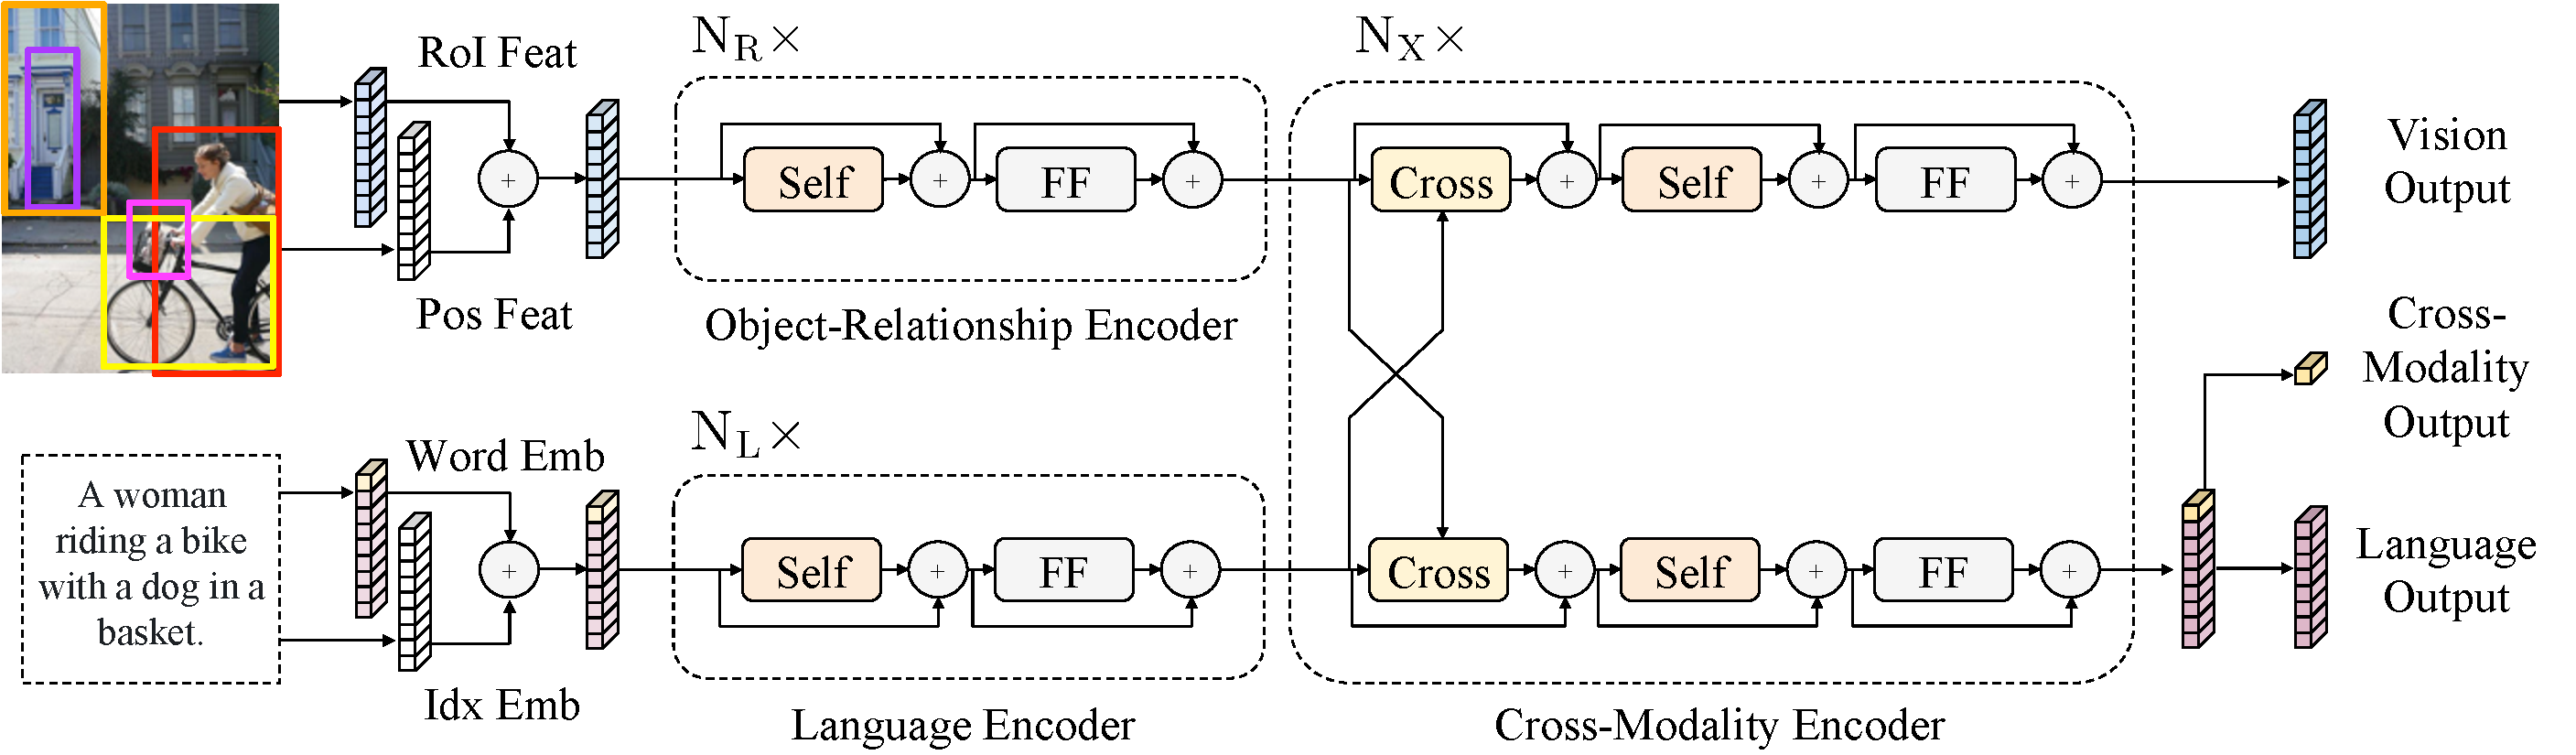
\includegraphics[width=\linewidth]{images/models/lxmert.pdf}
    \caption{The LXMERT model for learning vision-and-language cross-modality representations.}
    \label{fig:lxmert}
\end{figure}

\paragraph{VisualBERT.} VisualBERT \cite{li2019visualbert} aims to reuse transformer self-attention to align elements of the input text and regions in the input image (see \cref{fig:visualbert}). Visual embeddings are constructed by summing visual feature representation, segment embedding and position embeddings. Visual feature representations are obtained from a bounding region object detector. VisualBERT is trained using COCO using two objectives: masked language modelling (MLM) and sentence-image prediction task.

\begin{figure}[ht]
    \centering
    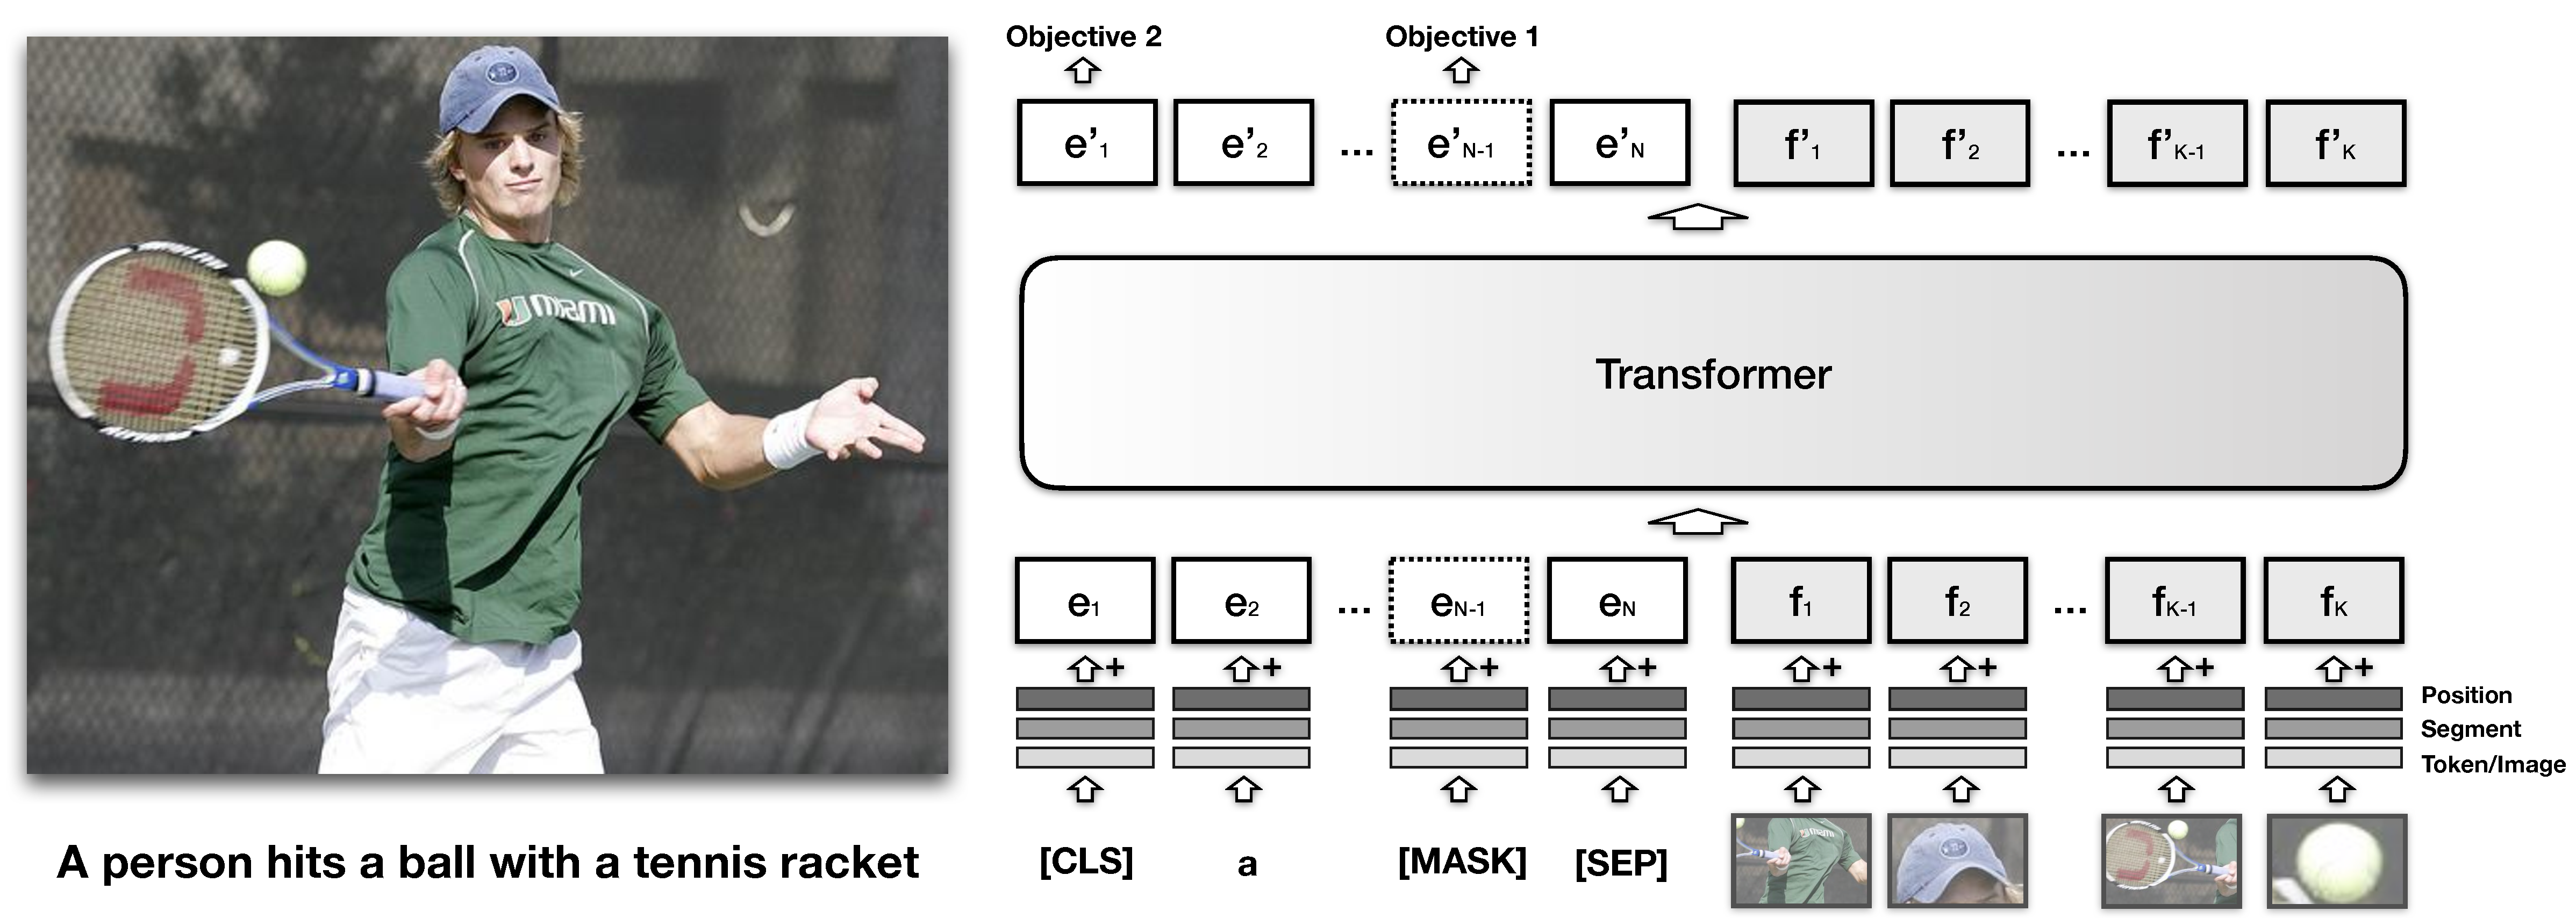
\includegraphics[width=\linewidth]{images/models/visualbert.pdf}
    \caption{The architecture of VisualBERT combines image regions and language with a transformer.}
    \label{fig:visualbert}
\end{figure}

\paragraph{UniT.} UniT \cite{hu2021unit} is a Unified Transformer model to simultaneously learn multiple tasks, such as object detection, natural language understanding and multimodal reasoning (see \cref{fig:unit}). UniT encodes each modality with an encoder and makes predictions on each task with a shared decoder and task-specific output heads. Model parameters are shared across all tasks instead of separately fine-tuning task-specific models.

\begin{figure}[ht]
    \centering
    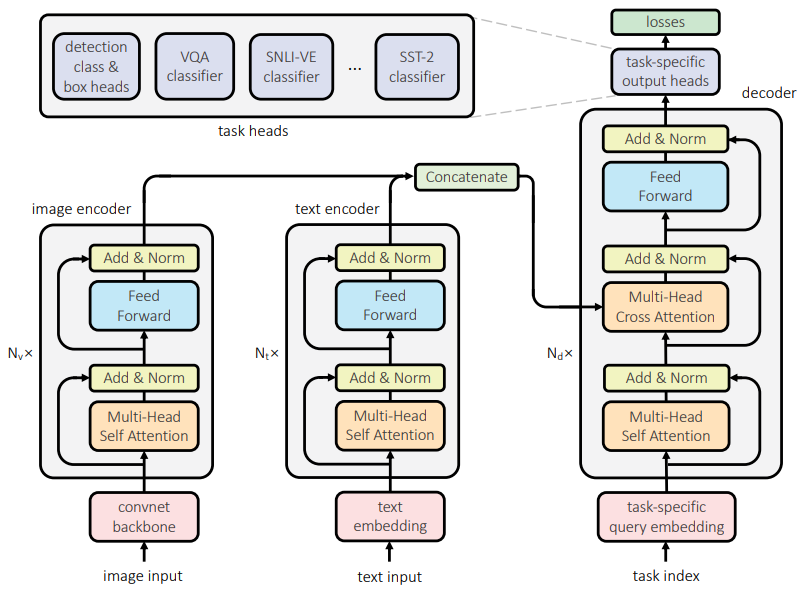
\includegraphics[width=\linewidth]{images/models/unit.png}
    \caption{An overview UniT, which jointly handles a wide range of tasks in different domains with a unified transformer encoder-decoder architecture.}
    \label{fig:unit}
\end{figure}

\paragraph{UNITER.} UNITER \cite{chen2020uniter} is a large-scale pre-trained model for joint multimodal embedding (see \cref{fig:uniter}). An Image Embedder is used to extract the visual features of each region and a Text Embedder to tokenize the input sentence. It is pre-trained using four image-text datasets: COCO, Visual Genome, Conceptual Captions, and SBU Captions. Four pretraining objectives were designed for this model: Masked Language Modeling (MLM), Masked Region Modeling (MRM), Image-Text Matching (ITM), and Word-Region Alignment (WRA).

\begin{figure}[ht]
    \centering
    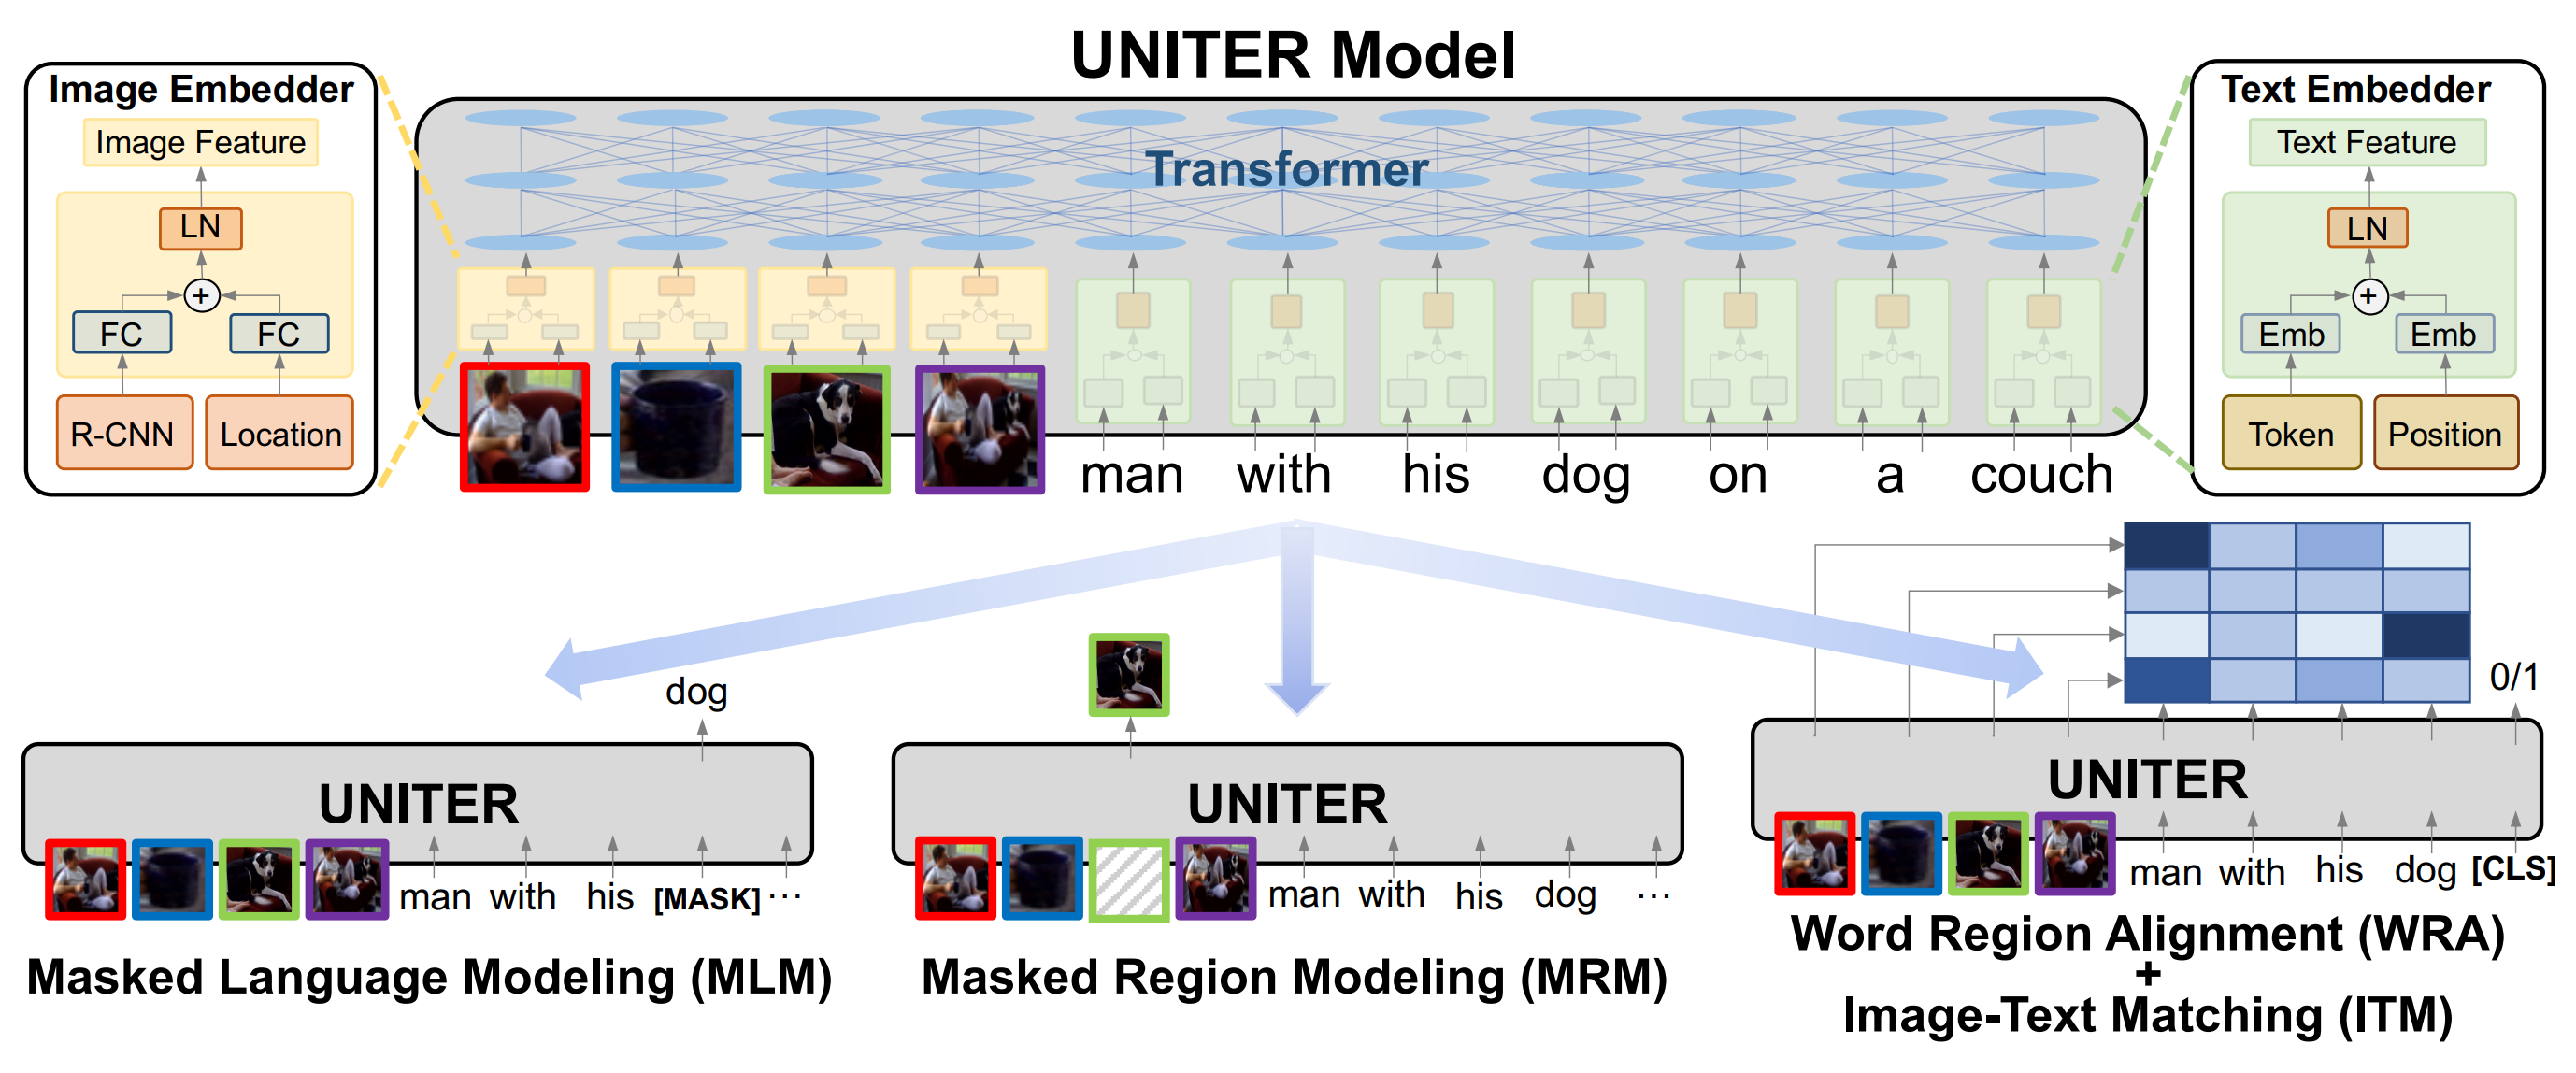
\includegraphics[width=\linewidth]{images/models/uniter.png}
    \caption{Overview of the UNITER model, consisting of an Image Embedder, a Text Embedder and a multi-layer Transformer}
    \label{fig:uniter}
\end{figure}

\paragraph{VILLA.} VILLA \cite{gan2020villa} is the first known effort on large-scale adversarial training for vision-and-language representation learning (see \cref{fig:villa}). VILLA consists of two training stages: task-agnostic adversarial pre-training and task-specific adversarial finetuning. Instead of adding adversarial perturbations on image pixels and textual tokens, it performs adversarial training in the embedding space of each modality. VILLA achieves SOTA on a wide range of tasks, including VQA, VCR, Image-Text Retrieval, Referring Expression Comprehension, Visual Entailment, and NLVR2.

\begin{figure}[ht]
    \centering
    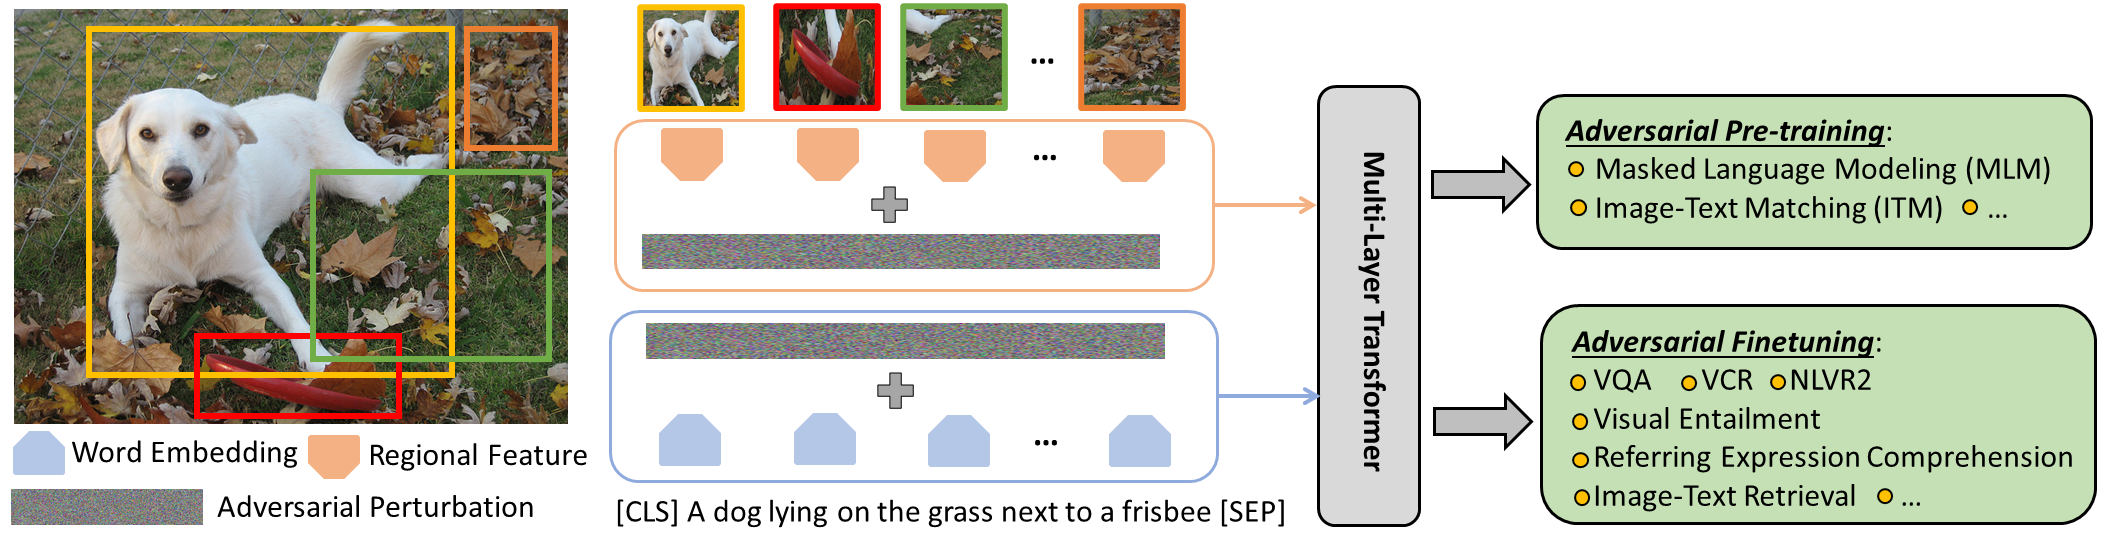
\includegraphics[width=\linewidth]{images/models/villa.png}
    \caption{Overview of the VILLA framework for vision-and-language representation learning.}
    \label{fig:villa}
\end{figure}

\paragraph{VinVL.} VinVL \cite{zhang2021vinvl} feeds the visual features generated by a new object detection model into a Transformer-based VL fusion model OSCAR \cite{li2020oscar} (see \cref{fig:oscar}). VinVL develops an improved object detection model to provide object-centric representations of images. The new visual features significantly improve the performance across all VL tasks, achieving state-of-the-art results.

\begin{figure}[ht]
    \centering
    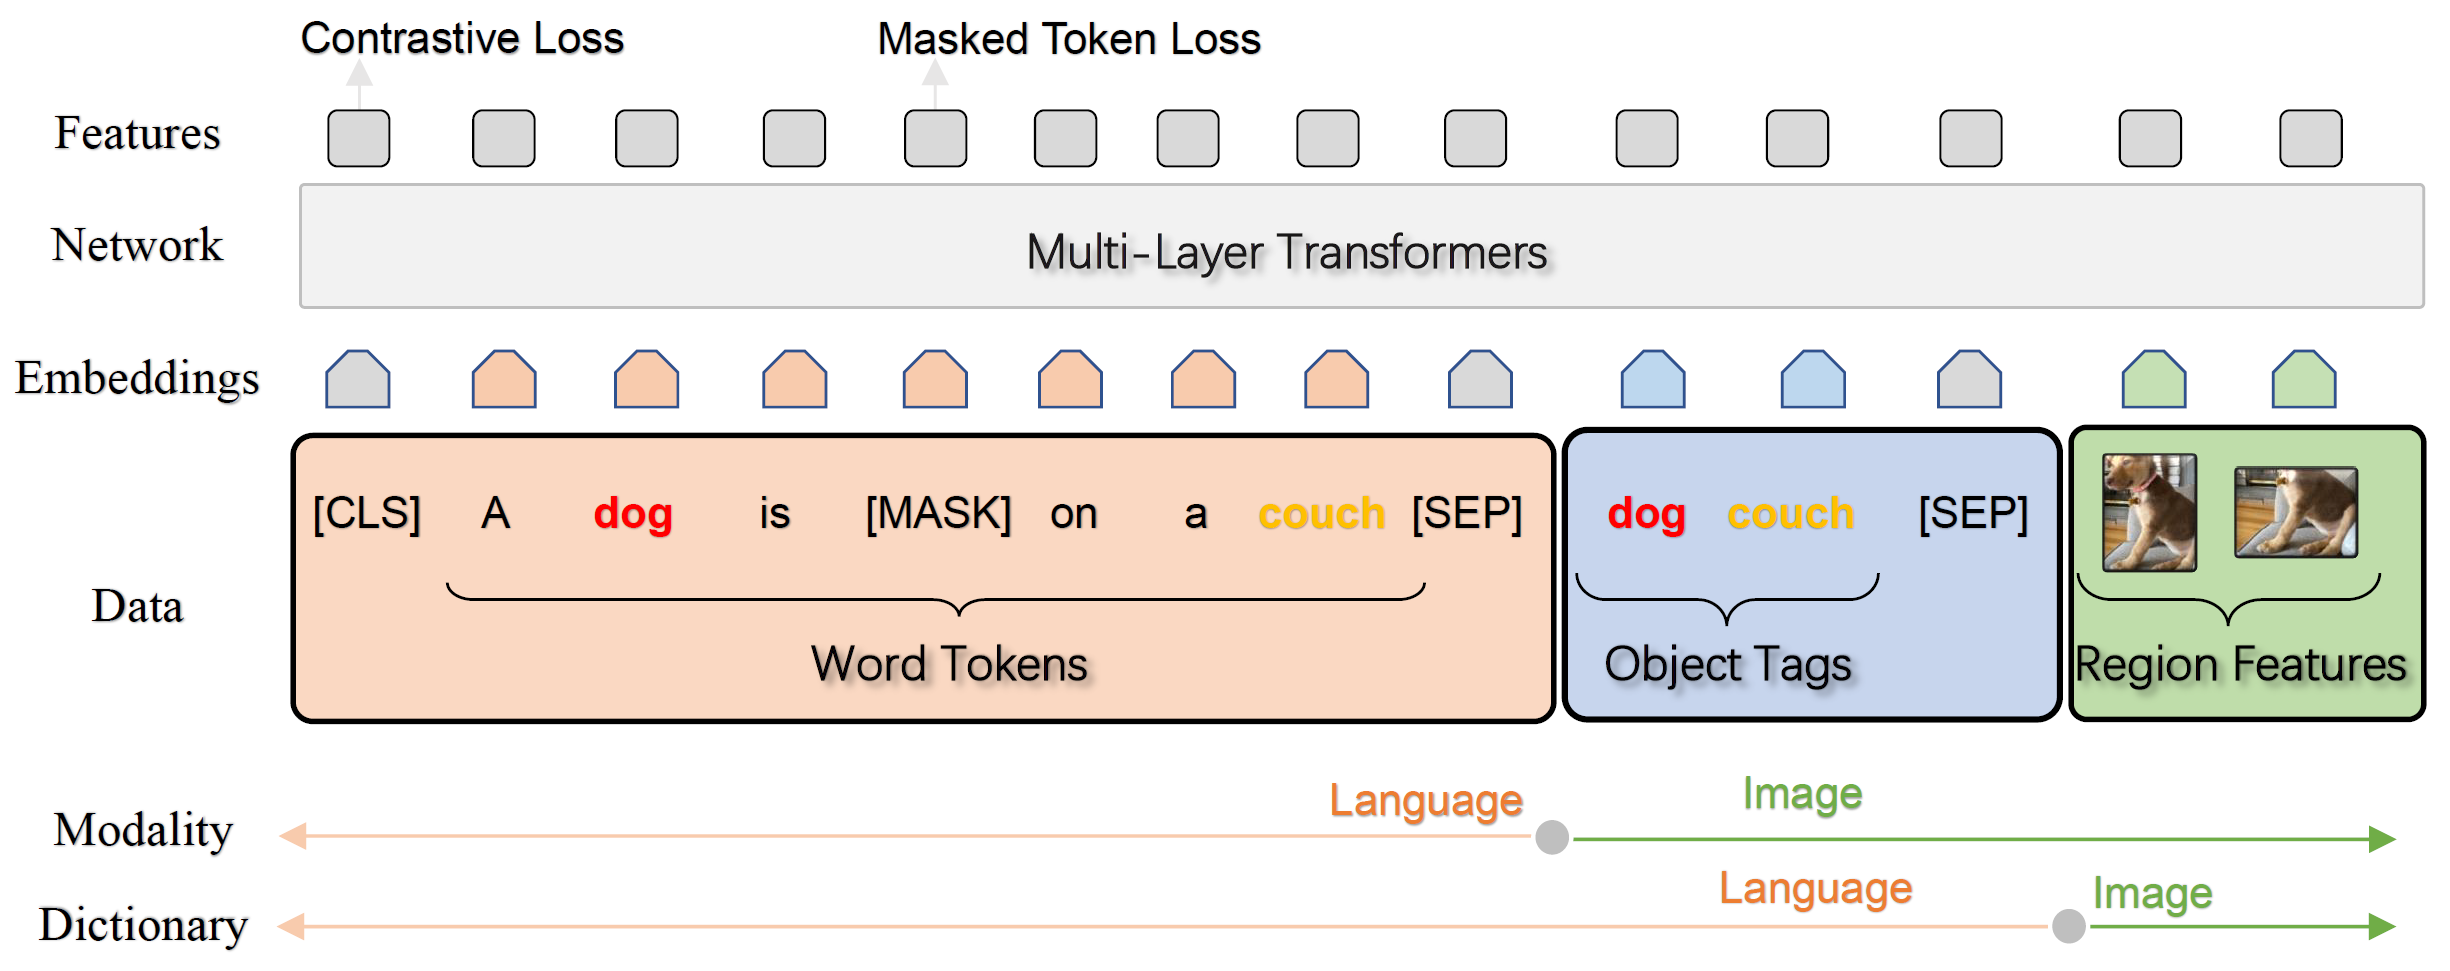
\includegraphics[width=\linewidth]{images/models/oscar.png}
    \caption{OSCAR model architecture that represents the image-text pair as a triple of word tokens, object tags and region features.}
    \label{fig:oscar}
\end{figure}

\paragraph{ViLBERT.} ViLBERT \cite{lu2019vilbert} is a BERT-based model for learning task-agnostic joint representations of images and language (see \cref{fig:vilbert}). ViLBERT extends the BERT architecture to a multi-modal model of two streams, which interact through co-attention transformer layers. ViLBERT is trained on the Conceptual Captions dataset under two training tasks: multi-modal learning and multi-modal alignment prediction.

\begin{figure}[ht]
    \centering
    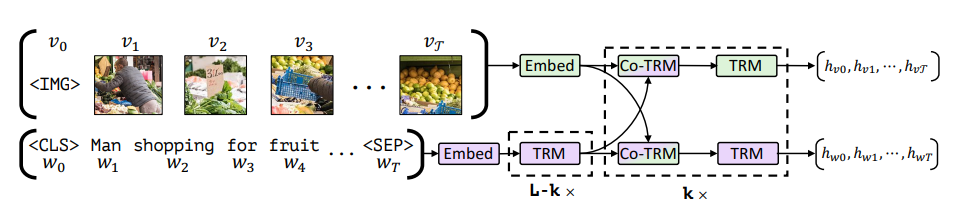
\includegraphics[width=\linewidth]{images/models/vilbert.png}
    \caption{ViLBERT model consists of two parallel streams for visual (green) and linguistic (purple) processing that interact through co-attentional transformer layers.}
    \label{fig:vilbert}
\end{figure}

\paragraph{ViLT.} ViLT \cite{kim2021vilt} is a minimal vision-and-language pre-training transformer model where the processing of visual inputs is simplified to the same way that text inputs are processed (see \cref{fig:vilt}). ViLT requires much less computation than previous VLMs and still gets good performance on downstream tasks. ViLT is pre-trained on the following objectives: image text matching (ITM), masked language modelling (MLM), and word patch alignment (WPA). It is fine-tuned on four downstream tasks: visual question answering (VQA2), visual reasoning (NLVR2) and image-text retrieval (COCO and Flickr30K).

\begin{figure}[ht]
    \centering
    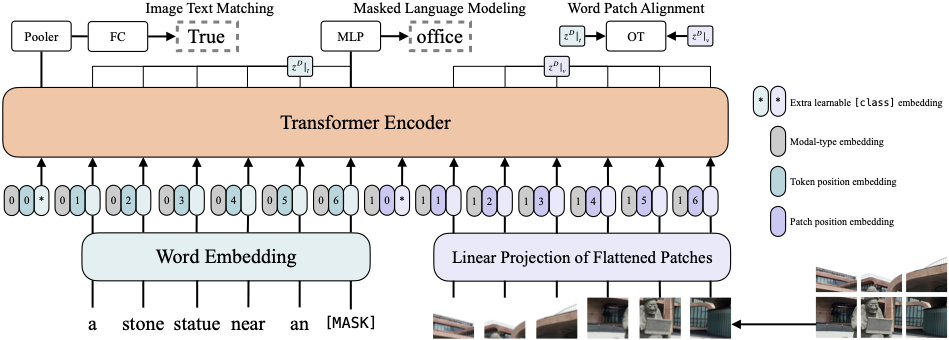
\includegraphics[width=\linewidth]{images/models/vilt.png}
    \caption{ViLT model overview.}
    \label{fig:vilt}
\end{figure}

\paragraph{FLAVA.} FLAVA \cite{singh2022flava} is a language vision alignment model that learns representations from multimodal and unimodal data. The model consists of three transformers, an image encoder, a text encoder and a multimodal encoder (see \cref{fig:flava}). During pretraining, masked image modelling (MIM) and mask language modelling (MLM), image-text contrastive (ITC), masked multimodal modelling (MMM), and image-text matching (ITM) objectives are used. Classification heads are applied to the outputs from the encoders for visual recognition, language understanding, and multimodal reasoning tasks.

\begin{figure}[ht]
    \centering
    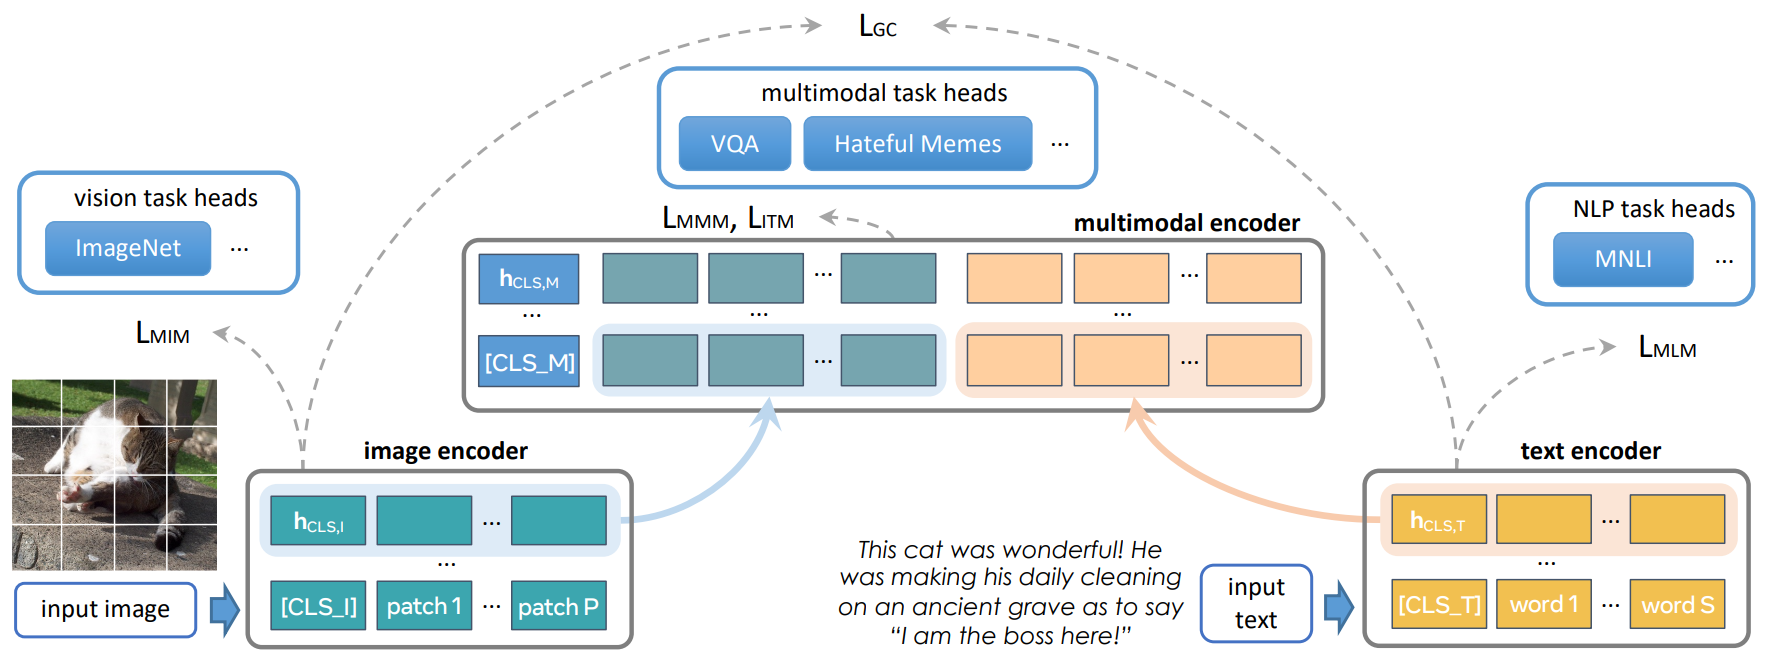
\includegraphics[width=\linewidth]{images/models/flava.png}
    \caption{FLAVA model overview.}
    \label{fig:flava}
\end{figure}

\paragraph{CLIP.} CLIP \cite{radford2021clip} models adopt two
unimodal encoders to get image and text representations (see \cref{fig:clip}). CLIP maximizes the similarity between positive image-text pairs, rendering strong unimodal representations. CLIP was trained by OpenAI on a closed dataset of 400M image-text pairs. CLIP variants use different visual backbones, including ViT-B/16, ViT-B/32, ViT-L/14, and ViT-L/14-336.

\begin{figure}[ht]
    \centering
    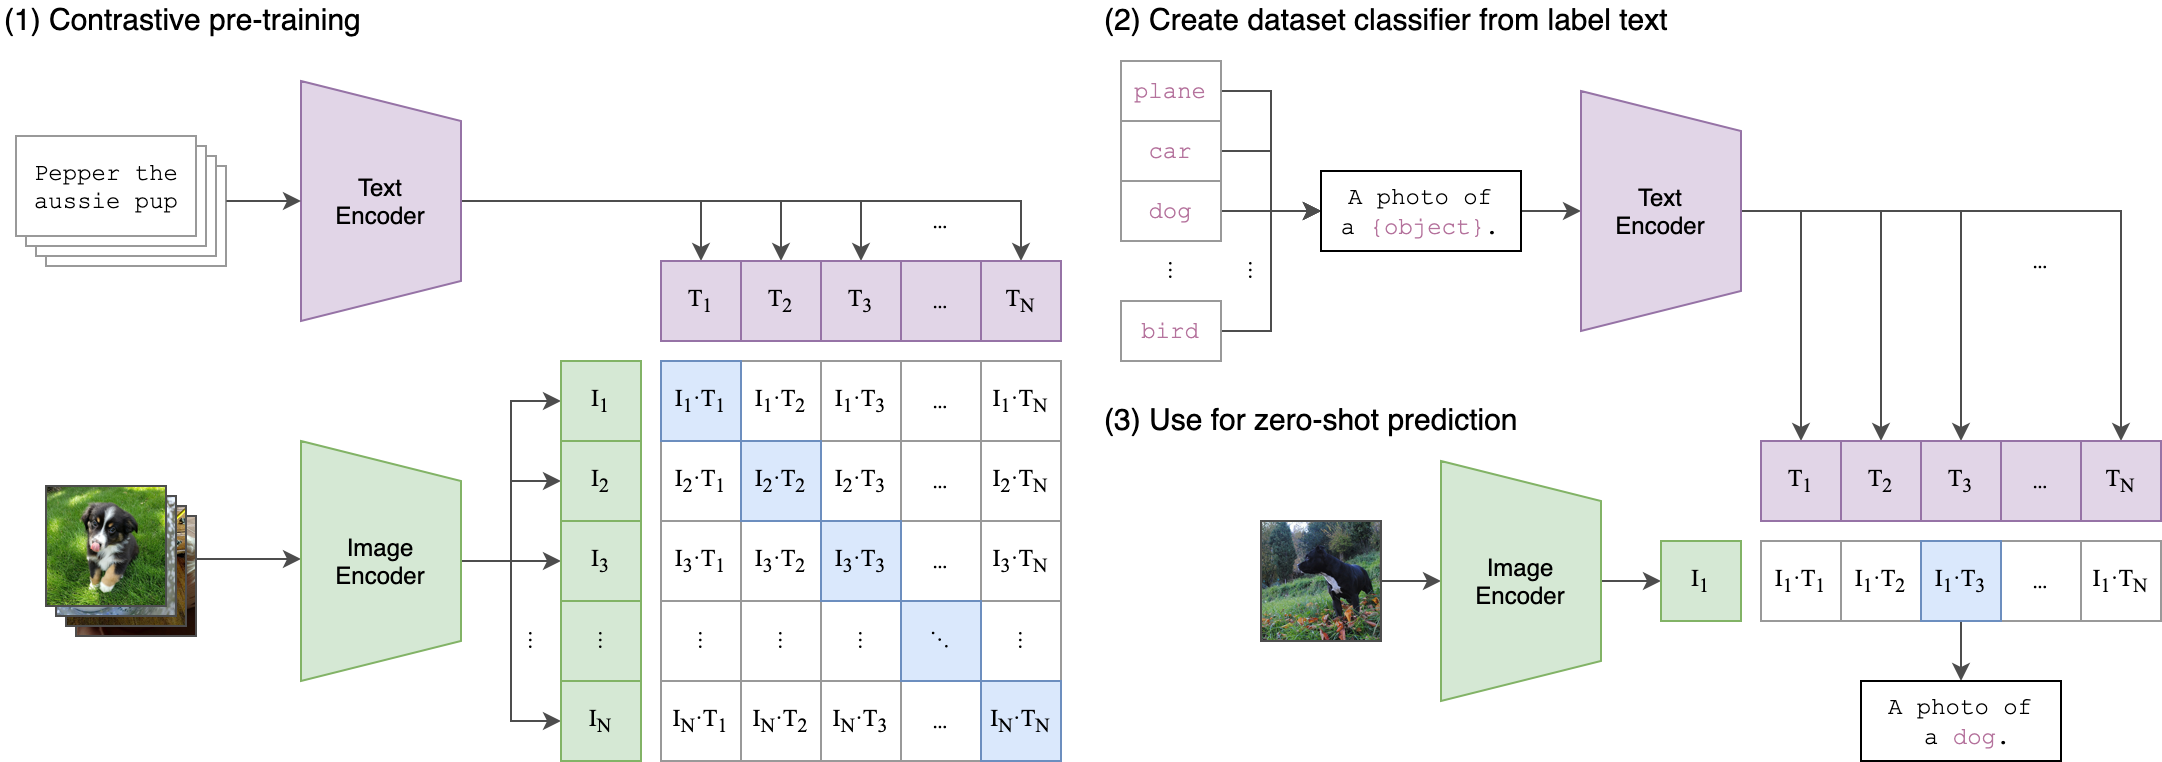
\includegraphics[width=\linewidth]{images/models/clip.png}
    \caption{CLIP model architecture.}
    \label{fig:clip}
\end{figure}

\paragraph{OpenCLIP.} OpenCLIP \cite{ilharco_gabriel_2021_5143773} models follow the same architecture (see \cref{fig:clip}), but are trained on LAION-2B, a subset of LAION-5B \cite{schuhmann2022laionb} with 2.32 billion English captions. There are different OpenCLIP variants depending on visual backbones: ViT-B/32, ViT-L/14, ViT-H/14, and ViT-g/14. The H/14 model achieves 78.0\% zero-shot top-1 accuracy on ImageNet and 73.4\% on zero-shot image retrieval at Recall@5 on MS COCO. This makes it the best open-source CLIP model.

\paragraph{BLIP.} BLIP \cite{li2022blip} achieves state-of-the-art performance on five vision-language tasks: image-text retrieval, image captioning, visual question answering, visual reasoning, and visual dialogue. It employs a Vision Transformer (ViT) \cite{dosovitskiy2020imageworth} as the image encoder and a BERT as the text encoder. BLIP proposes a mixture of encoder-decoder (MED), which can operate either as a unimodal image or text encoder, an image-grounded text encoder, or an image-grounded text decoder (see \cref{fig:blip}). This enables both multimodal understanding and generation. Moreover, BLIP proposes dataset bootstrapping to improve the quality of the pretraining captions by removing noisy ones and generating new ones. BLIP is jointly pretrained with three objectives: language modeling (LM), image-text contrastive learning (ITC) and image-text matching (ITM). There are BLIP variants that use different vision transformers: ViT-B/16 and ViT-L/16. Fine-tuned checkpoints are also available for many downstream tasks.

\begin{figure}[ht]
    \centering
    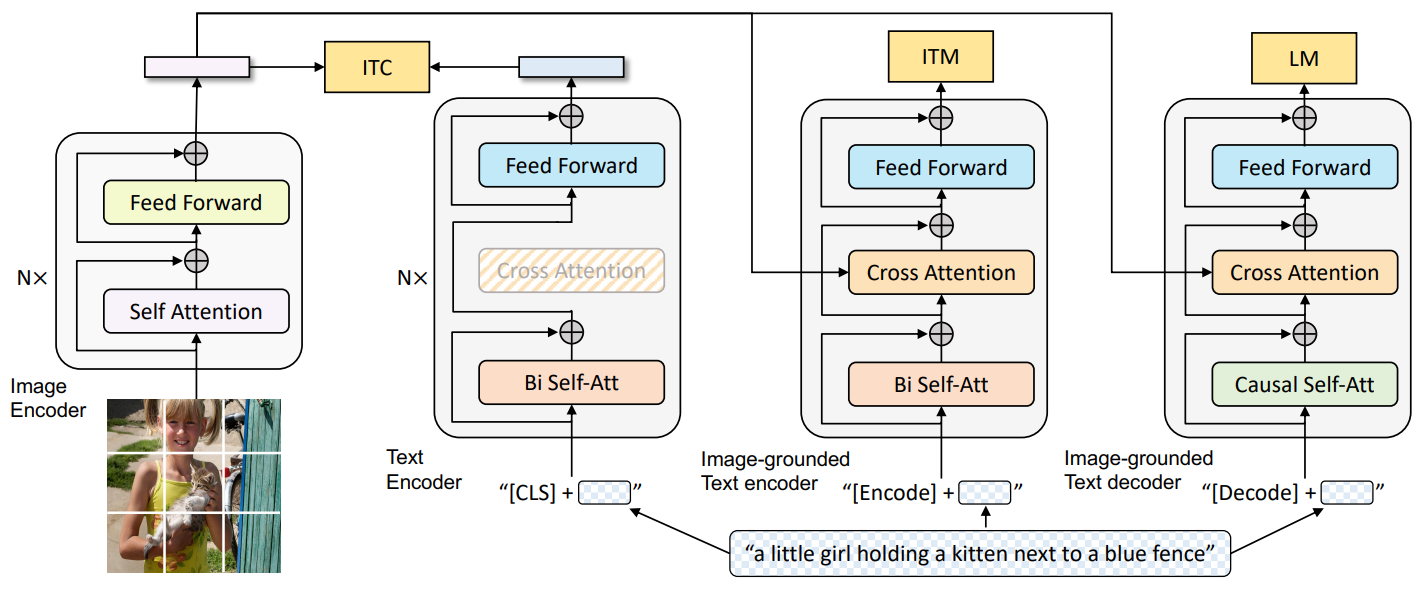
\includegraphics[width=\linewidth]{images/models/blip.png}
    \caption{BLIP pre-training model architecture: a multimodal mixture
of encoder-decoder (MED).}
    \label{fig:blip}
\end{figure}

\paragraph{OFA.} OFA \cite{wang2022unifying} is a sequence-to-sequence pretrained model that unifies modalities and tasks. It performs a lot of cross-modal and uni-modal tasks, including image generation, visual grounding, image captioning, image classification and language modelling (see \cref{fig:ofa}). In contrast with the recent VLMs that require large cross-modal datasets, OFA is pretrained on only 20M publicly available image-text pairs. Despite this, OFA achieves SOTA in various cross-modal tasks and competitive performance on uni-modal tasks.

\begin{figure}[ht]
    \centering
    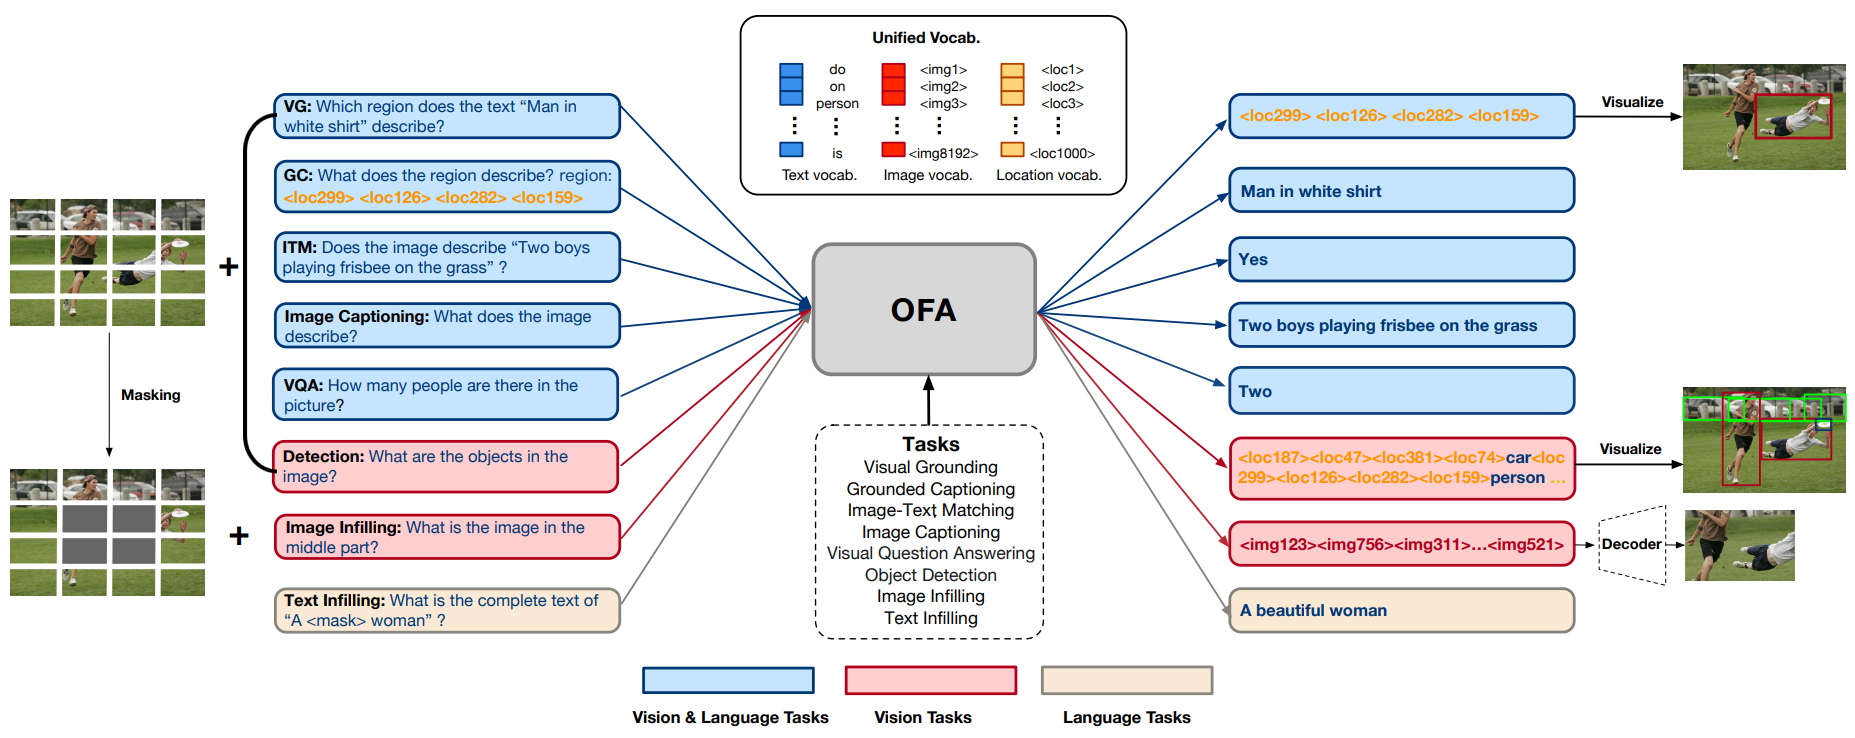
\includegraphics[width=\linewidth]{images/models/ofa.png}
    \caption{OFA pretraining tasks: visual grounding, grounded captioning, image-text matching, image captioning, VQA, object detection, image infilling and text infilling.}
    \label{fig:ofa}
\end{figure}

\subsection{Multimodal RNNs} \label{sec:multimodal_rnns}

Multimodal RNNs were the SOTA approach for vision-language tasks before transformers. Two sequence-based models are included in Winoground \cite{thrush2022winoground} evaluation, VSE++ \cite{faghri2018vse} and VSRN \cite{li2019vsrn}. Both models minimize the hardest negative score. which is the highest-scoring image-caption pair that is not correct. Both models use a GRU\ cite{chung2014gru} to get language embeddings.

\paragraph{VSE++.} VSE++ \cite{faghri2018vse} uses a new technique for learning visual-semantic embeddings for cross-modal
retrieval, and is based on VSE (see \cref{fig:vse}). VSE's image encoder is a linear projection of the embedding from a backbone (either ResNet152 \cite{he2016deep} or VGG19 \cite{simonyan2015very}). VSE++ is trained on COCO and Flickr30K datasets, obtaining state-of-the-art results on image-text retrieval.

\begin{figure}[ht]
    \centering
    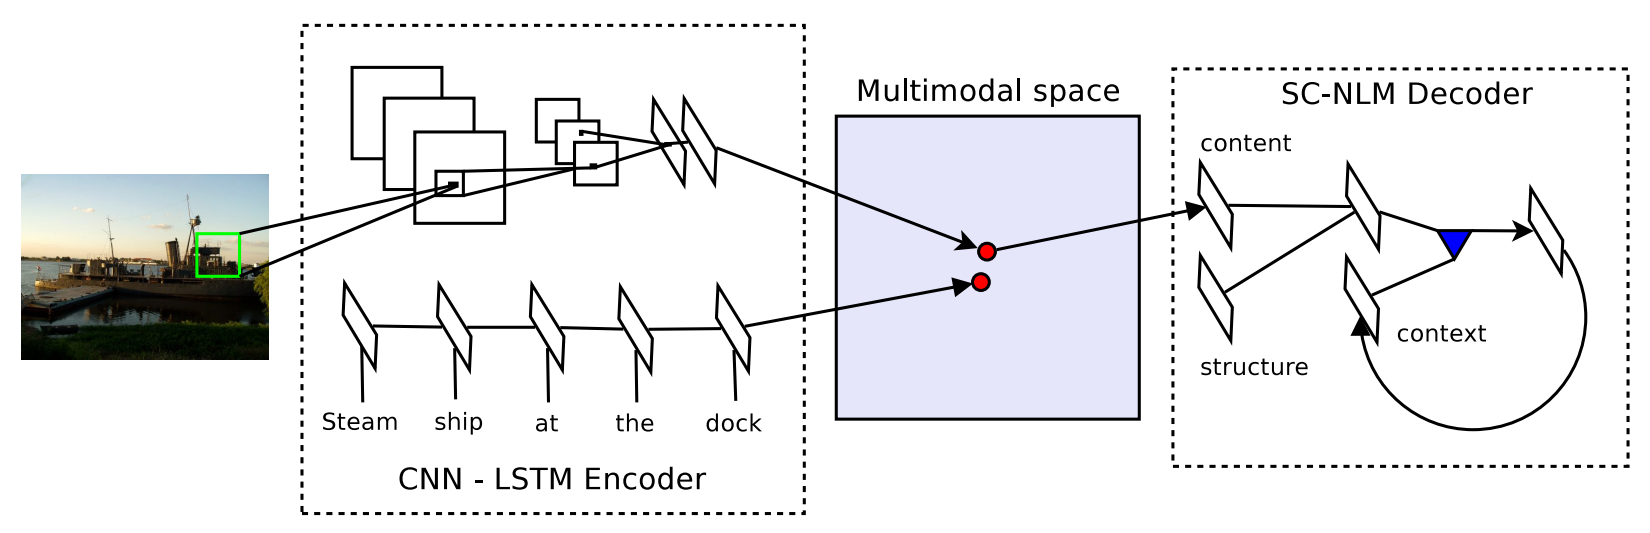
\includegraphics[width=\linewidth]{images/models/vse.png}
    \caption{VSE model architecture. The encoder is composed of a CNN and an LSTM for learning a joint image-sentence embedding. The decoder is an NLM that combines structure and content vectors for generating words one by one.}
    \label{fig:vse}
\end{figure}

\paragraph{VSRN.} VSRN \cite{li2019vsrn} is a simple and interpretable reasoning model to generate a visual representation that captures key objects and semantic concepts of a scene (see \cref{fig:vsrn}). A Faster R-CNN is used to get a sequence of features which are fed into a GRU to obtain image embeddings. VSRN is trained on COCO and Flickr30K datasets, outperforming previous models on image-text retrieval.

\begin{figure}[ht]
    \centering
    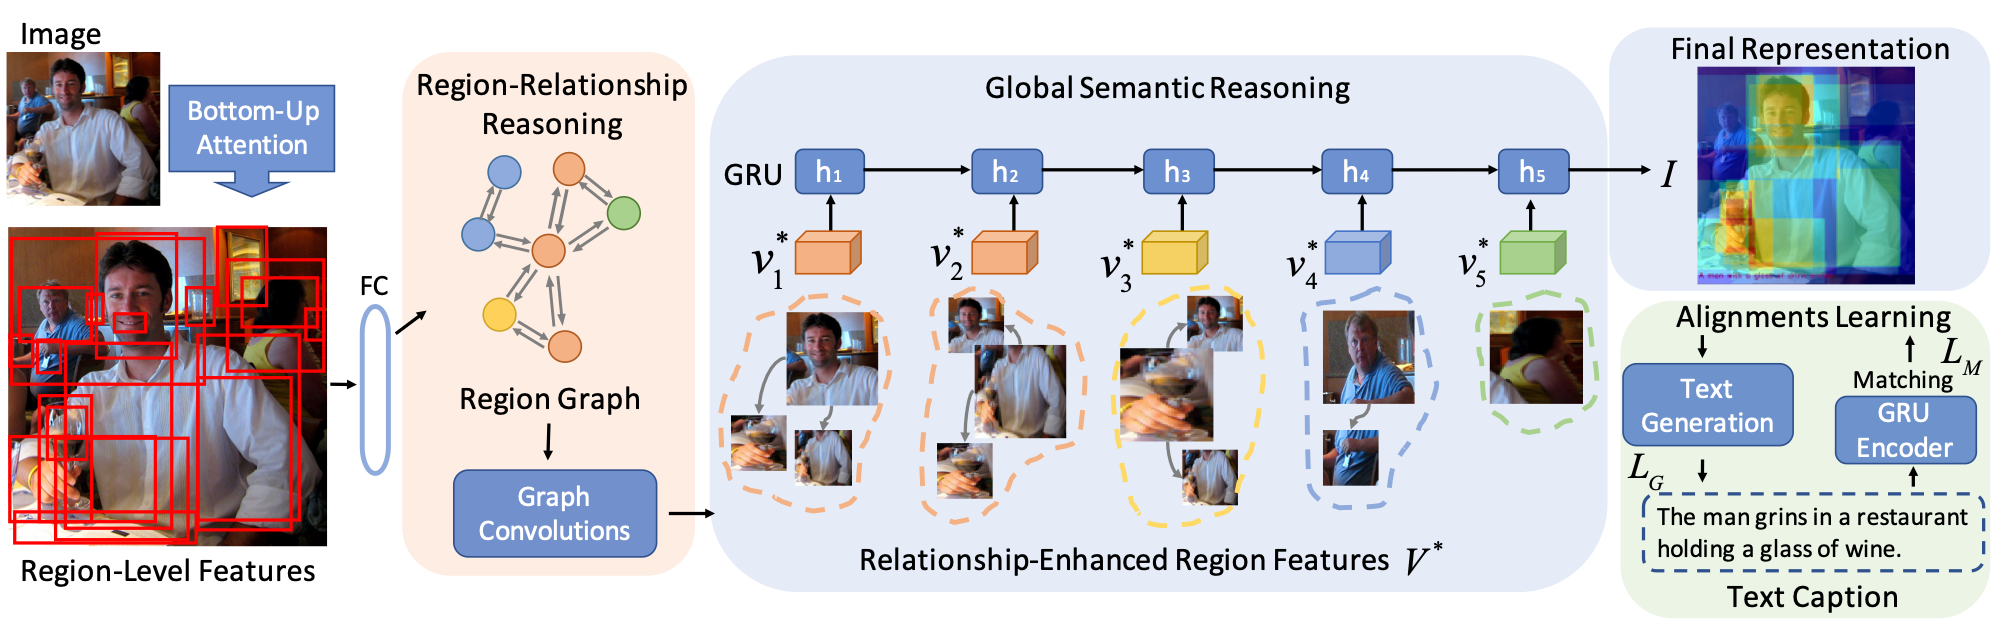
\includegraphics[width=\linewidth]{images/models/vsrn.png}
    \caption{An overview of VSRN (Visual Semantic Reasoning Network).}
    \label{fig:vsrn}
\end{figure}

\subsection{Diffusion Models} \label{sec:diffusion_models}

Diffusion models are trained to denoise random gaussian noise step by step, to get a sample image. Neural networks are trained to predict a way to slightly denoise the picture in each step. As we can see in \cref{fig:diffusion_process}, after a certain number of steps, a sample is obtained.

\begin{figure}[ht]
    \centering
    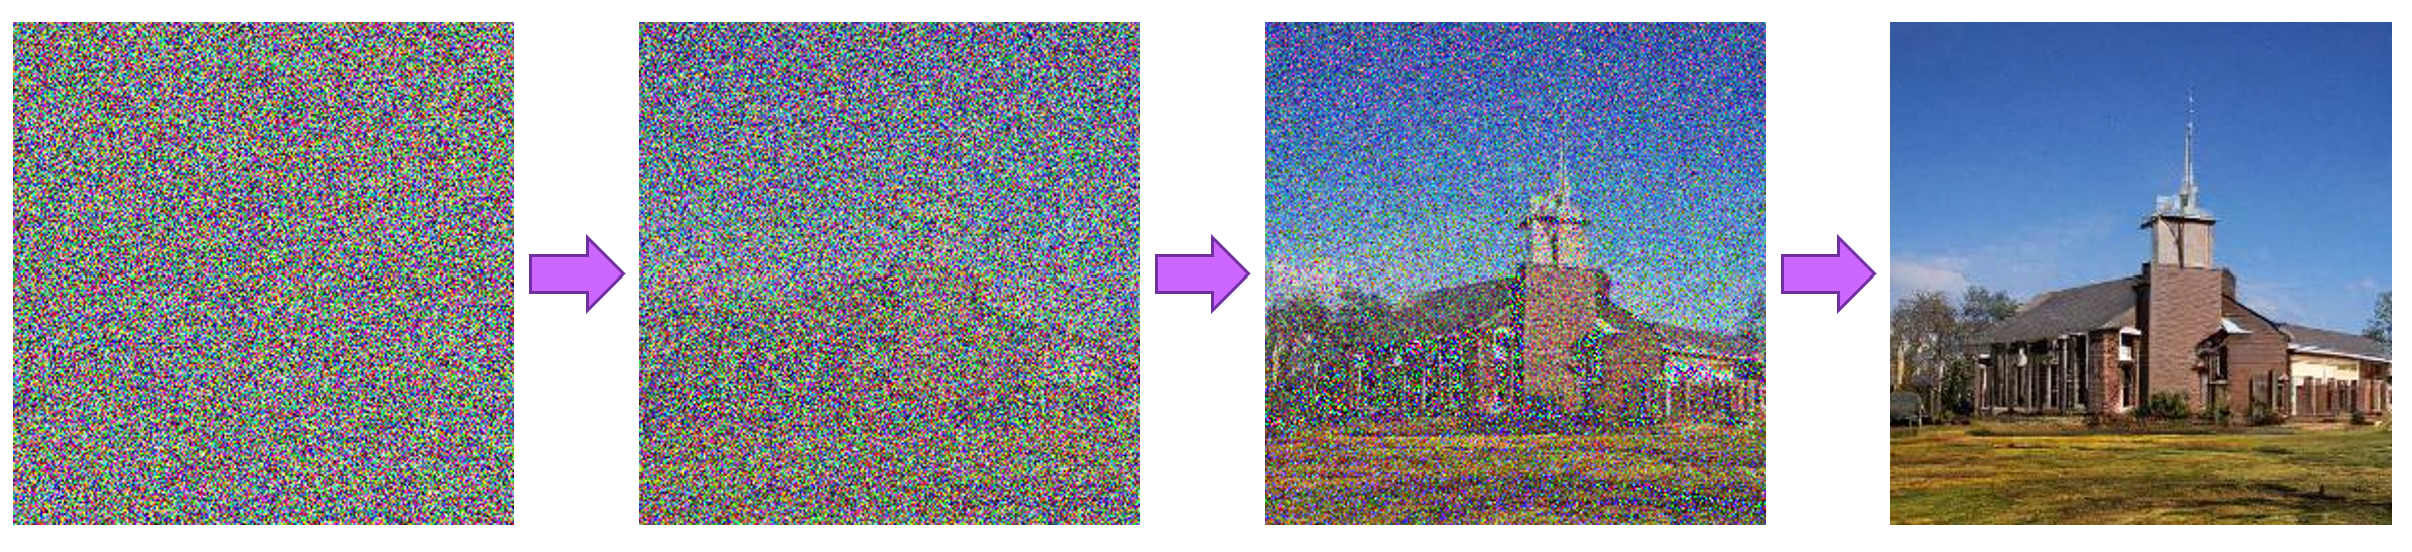
\includegraphics[width=\linewidth]{images/diffusion/diffusion-process.png}
    \caption{In the diffusion process random images are denoised in multiple steps to get a sample image.}
    \label{fig:diffusion_process}
\end{figure}

Diffusion models have obtained SOTA results on image generation. However, one downside of diffusion models is that the reverse denoising process is slow. In addition, these models consume a lot of memory because they work in pixel space. Therefore, it is challenging to train these models and also to use them for inference.

Consequently, most of the recent diffusion models, e.g. DALLE-2 \cite{ramesh2022hierarchical} and IMAGEN \cite{saharia2022photorealistic}, are unfortunately not accessible to the community. The most popular exception is Stable Diffusion \cite{rombach2021highresolution}, which has been open sourced and can be used on a single GPU.

\paragraph{Stable Diffusion.}

Stable Diffusion is based on a type of diffusion model called Latent Diffusion \cite{rombach2021highresolution}. Latent diffusion reduces the memory and compute complexity by applying the diffusion process over a lower dimensional latent space. There are three main components in latent diffusion: an autoencoder (VAE), a U-Net and a text-encoder (CLIP).

\textbf{The autoencoder (VAE).} The VAE \cite{kingma2013auto} has two parts, an encoder and a decoder, as we can see in \cref{fig:vae}. During latent diffusion training, the encoder maps the images to a latent space for the forward diffusion process, which applies more noise at each step. During inference, the decoder maps the latents generated by the reverse diffusion process back to the images. The encoder and decoder are trained jointly to minimize the reconstruction error.

\begin{figure}[ht]
    \centering
    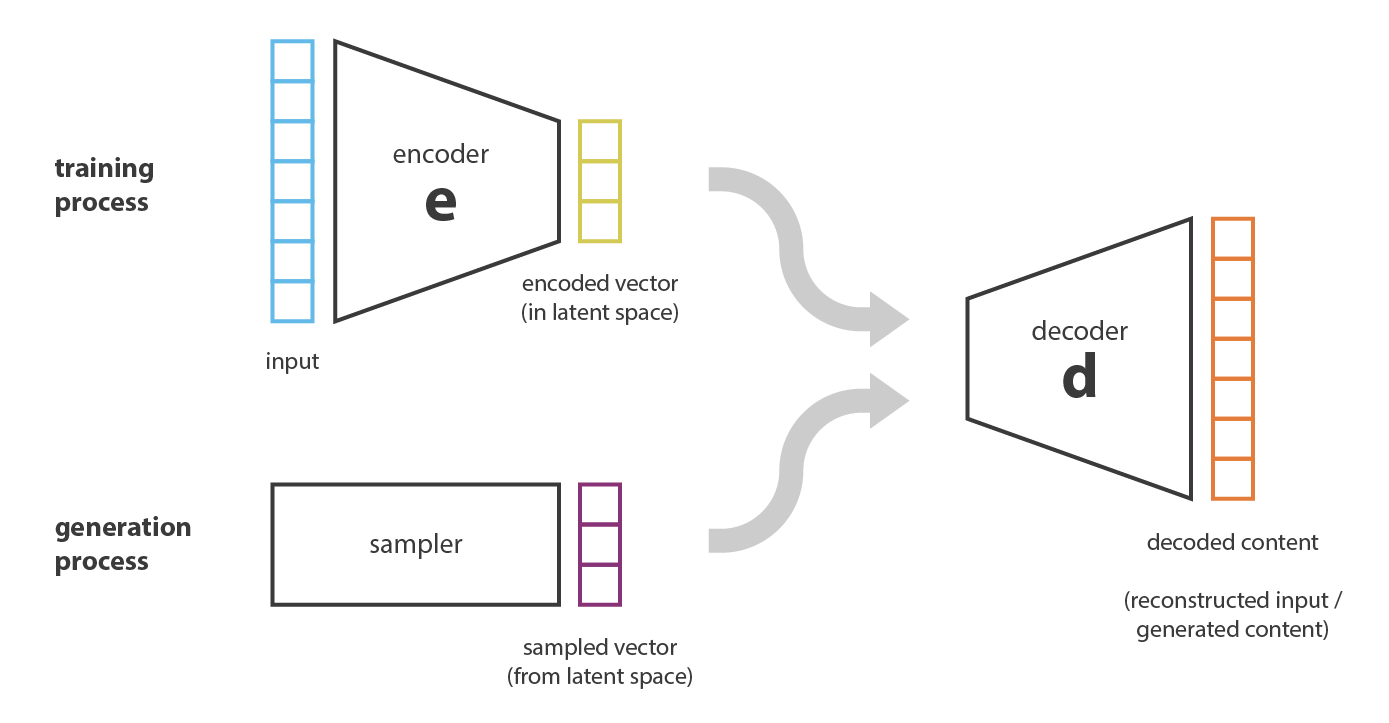
\includegraphics[width=\linewidth]{images/diffusion/vae.png}
    \caption{Variational Autoencoder (VAE) training and generation processes.}
    \label{fig:vae}
\end{figure}

\textbf{The U-Net.} The U-Net \cite{ronneberger2015u} also has an encoder part and a decoder part, as shown in \cref{fig:unet_model}. The encoder has several ResNet blocks which half the image size by 2. The decoder does the opposite process to upsample the image to the initial size. The U-Net outputs the noise residual which can be used to compute the denoised image representation. To prevent the U-Net from losing important information while downsampling, shortcut connections are usually added from the downsample path to the corresponding layers in the upsample path. Moreover, the output of the stable diffusion U-Net is conditioned on text-embeddings via cross-attention layers.

\begin{figure}[ht]
    \centering
    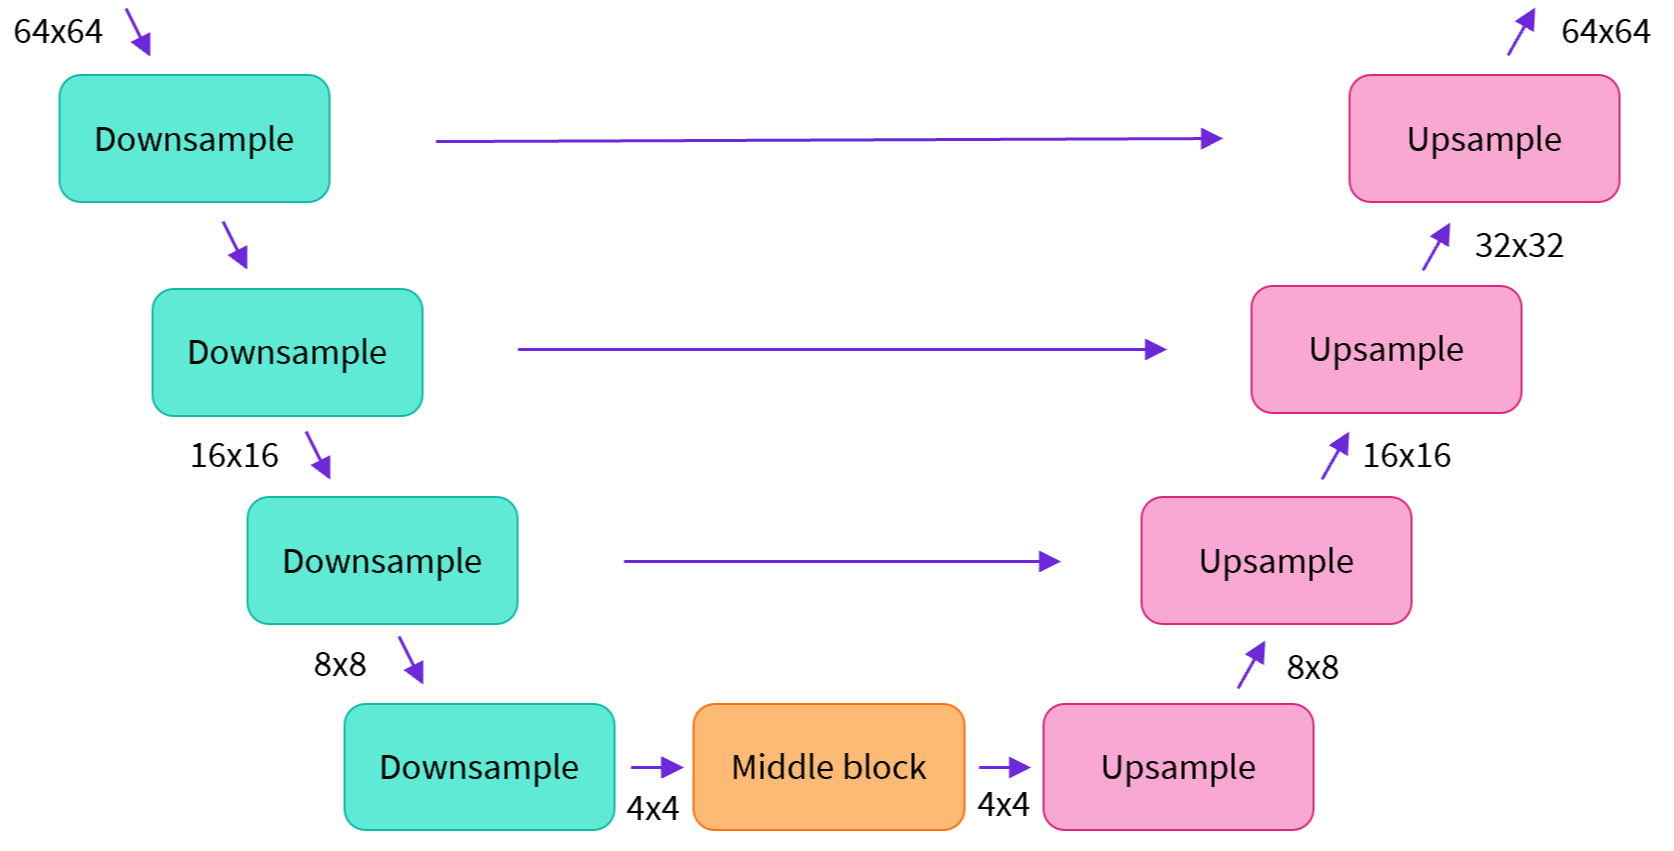
\includegraphics[width=\linewidth]{images/diffusion/unet-model.png}
    \caption{The architecture of the U-Net model.}
    \label{fig:unet_model}
\end{figure}

\textbf{The text-encoder (CLIP).} The CLIP \cite{radford2021clip} text-encoder transforms the input prompt into an embedding for the U-Net. Stable Diffusion does not train the text-encoder during training and uses an already trained CLIP text encoder.

With the previous components we nearly have the full Stable Diffusion inference architecture \cref{fig:stable_diffusion}. The stable diffusion model takes a latent seed and a text prompt as input. The latent seed is  used to generate initial random latents. The output of the U-Net is used to compute a denoised image representation with a scheduler algorithm. This process is repeated many to get better representations in each iteration. Finally, the latent image representation is decoded by the VAE decoder.

\begin{figure}[ht]
    \centering
    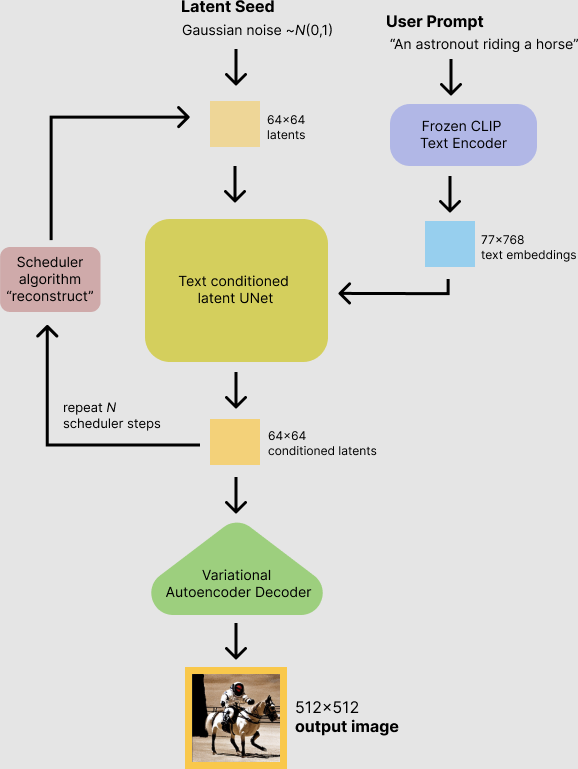
\includegraphics[width=0.6\linewidth]{images/diffusion/stable_diffusion.png}
    \caption{Stable Diffusion inference architecture.}
    \label{fig:stable_diffusion}
\end{figure}

\section{Visual Reasoning Datasets} \label{sec:visual_reasoning_datasets}

This section includes information about visual reasoning datasets. Sections \ref{sec:synthetic_visual_reasoning_datasets} and \ref{sec:natural_visual_reasoning_datasets} introduce some of the existing Synthetic and Natural Visual Reasoning Datasets. \cref{sec:compositional_spatial_reasoning_datasets} explains the two datasets that we have chosen for Compositional and Spatial Reasoning.

\subsection{Synthetic Visual Reasoning Datasets} \label{sec:synthetic_visual_reasoning_datasets}

Multimodal training datasets with images and descriptions that include spatial relations tend to be small. Synthetic visual reasoning datasets have been proposed to overcome this problem. These datasets enable full control of dataset generation, easing spatial reasoning capability probing  on VLMs. Some examples of synthetic datasets include SHAPES \cite{andreas2016neural}, CLEVR \cite{johnson2017clevr}, NLVR \cite{suhr-etal-2017-corpus} and SPARTQA \cite{mirzaee-etal-2021-spartqa}.

\textbf{SHAPES} is a dataset of synthetic images designed to benchmark understanding of spatial and logical relations among multiple objects \cite{andreas2016neural}. The dataset consists of complex yes or no questions about arrangements of colored shapes. Each image is a 3×3 grid of objects. Each object is characterized by shape (circle, square, triangle), colour (red, green, blue) and size (small, big). \cref{fig:shapes_examples} shows some example images and questions.

\begin{figure}[ht]
  \centering
    \begin{subfigure}[b]{0.24\linewidth}
    \centering
    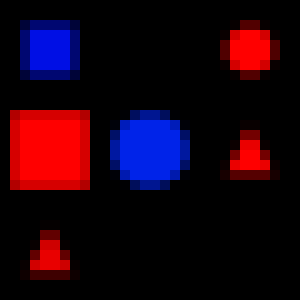
\includegraphics[width=\linewidth]{images/datasets/shapes0_big.png}
    \caption{\textbf{Q:} is a red shape blue? \\ \textbf{A:} no}
     \end{subfigure}
     \hfill
     \begin{subfigure}[b]{0.24\linewidth}
     \centering
    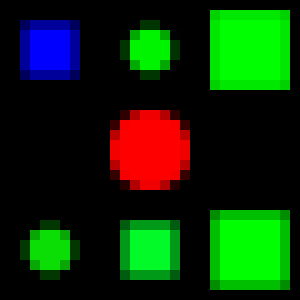
\includegraphics[width=\linewidth]{images/datasets/shapes1_big.png}
    \caption{\textbf{Q:} is there a blue shape below a square? \textbf{A:} no}
     \end{subfigure}
     \hfill
     \begin{subfigure}[b]{0.24\linewidth}
    \centering
    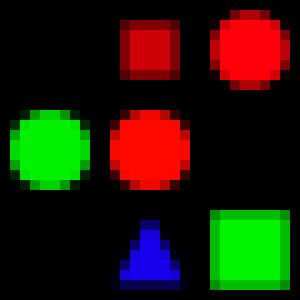
\includegraphics[width=\linewidth]{images/datasets/shapes2_big.png}
    \caption{\textbf{Q:} is there a red shape above a circle? \textbf{A:} yes}
     \end{subfigure}
     \hfill
     \begin{subfigure}[b]{0.24\linewidth}
     \centering
    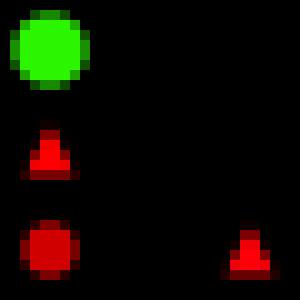
\includegraphics[width=\linewidth]{images/datasets/shapes3_big.png}
    \caption{\textbf{Q:} is there a red shape below a triangle? \textbf{A:} yes}
     \end{subfigure}
    \caption{Example images, questions and answers from SHAPES.}
    \label{fig:shapes_examples}
\end{figure}

\textbf{CLEVR} was one of the pioneering works on testing \textbf{compositional language and elementary visual reasoning} \cite{johnson2017clevr}. However, it presents two major drawbacks: i) questions not only cover spatial grounding but some other concepts such as compositional language and attribute identification, and ii) spatial relations are limited to four, i.e. left, right, behind and in front. A sample image and questions are shown in \cref{fig:clevr_example}.

\begin{figure}[ht]
  \centering
  \begin{minipage}{0.49\textwidth}
  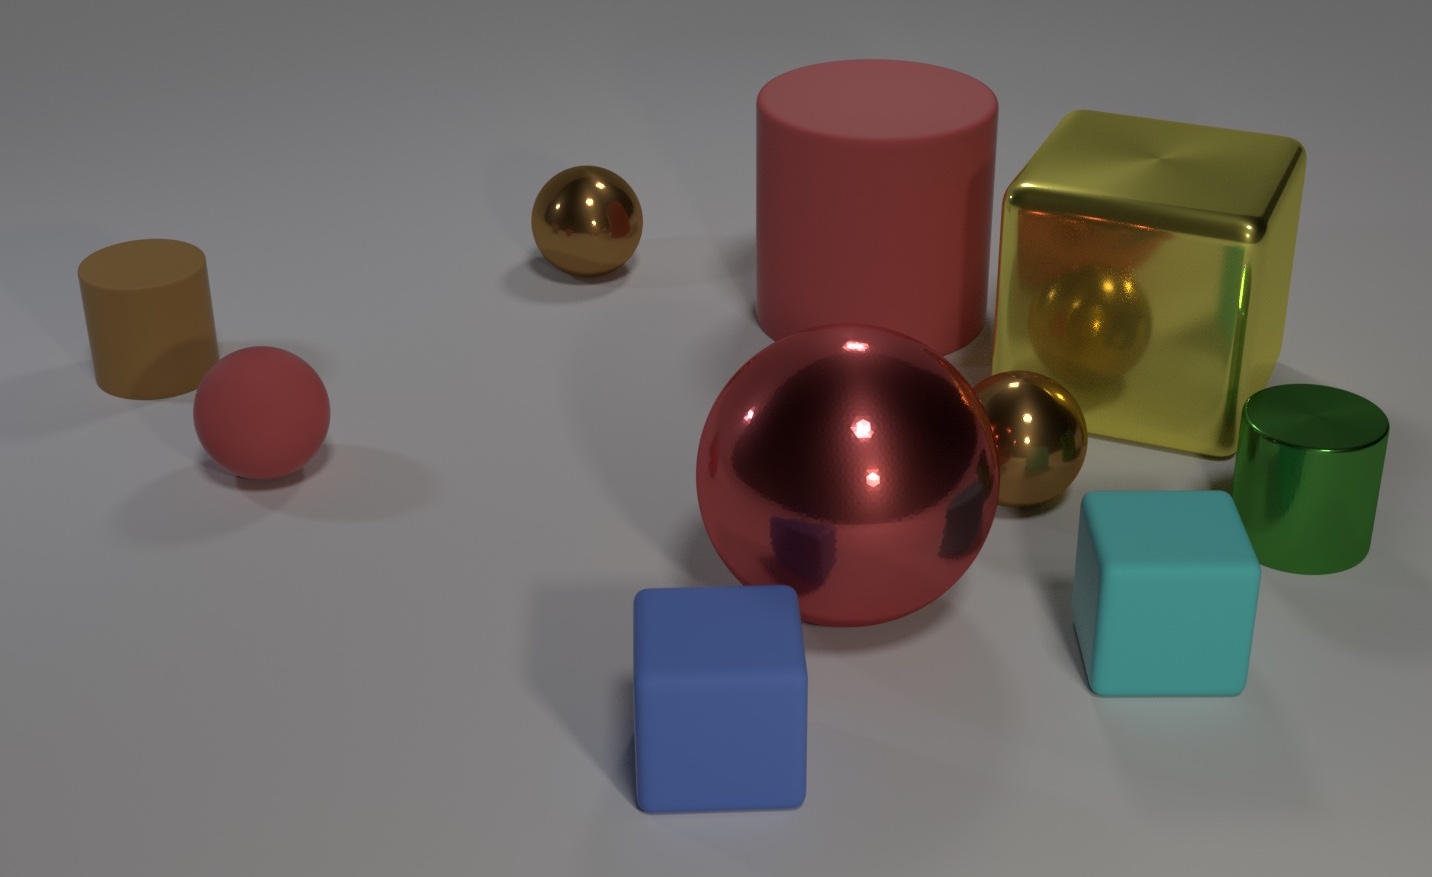
\includegraphics[width=\textwidth]{images/datasets/clevr_example.jpg}
  \end{minipage}
  \vspace{1mm}
  \begin{minipage}{0.49\textwidth}
    \footnotesize
    \textbf{Q:} Are there an \textcolor{blue}{equal} \textcolor{red}{number} of
    \textcolor{brown}{large} things and \textcolor{brown}{metal spheres}? \textbf{A:} no \\\\
    \textbf{Q:} \textcolor{brown}{What size} is the \textcolor{brown}{cylinder}
    \textcolor{green}{that is left of} the \textcolor{brown}{brown metal} thing
    \textcolor{green}{that is left of} the \textcolor{brown}{big sphere}? \textbf{A:} small \\\\
    \textbf{Q:} There is a \textcolor{brown}{sphere} with the \textcolor{blue}{same size as}
    the \textcolor{brown}{metal cube}; is it
    \textcolor{blue}{made of the same material as} the \textcolor{brown}{small red sphere}? \textbf{A:} no \\\\
    \textbf{Q:} \textcolor{red}{How many} objects \textcolor{purple}{are either}
    \textcolor{brown}{small cylinders}
    \textcolor{purple}{or} \textcolor{brown}{metal} things? \textbf{A:} 6
  \end{minipage}
  \vspace{1mm}
  \caption{A sample image, questions and answers from CLEVR. Questions test aspects of visual reasoning
    such as \textcolor{brown}{attribute identification}, \textcolor{red}{counting},
    \textcolor{blue}{comparison}, \textcolor{green}{spatial relations},
    and \textcolor{purple}{logical operations}.
  }
  \vspace{-4mm}
  \label{fig:clevr_example}
\end{figure}

\textbf{NLVR} contains natural language sentences grounded in images \cite{suhr-etal-2017-corpus}. The task is to determine whether a sentence is true about a visual input. The data was collected through crowdsourcing, and solving the task requires reasoning about sets of objects, comparisons, and spatial relations. \cref{fig:nlvr_examples} shows two examples from NLVR.

\begin{figure}[ht]
  \centering
    \centering
    \begin{subfigure}[b]{0.49\linewidth}
    \centering
    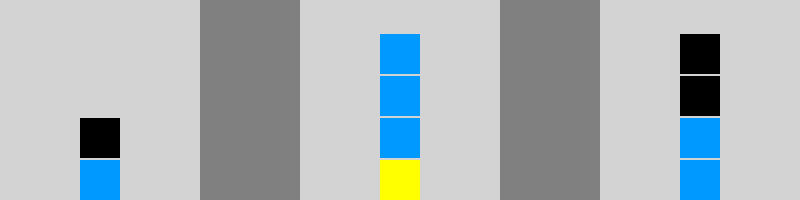
\includegraphics[width=\linewidth]{images/datasets/nlvr_ex_0.png}
    \caption{There is at least one tower with four blocks with a yellow block at the base and a blue block below the top block.}
     \end{subfigure}
     \hfill
     \begin{subfigure}[b]{0.49\linewidth}
     \centering
    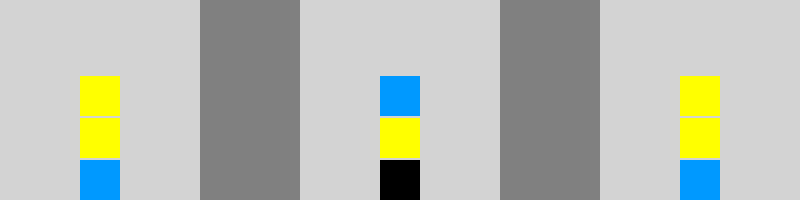
\includegraphics[width=\linewidth]{images/datasets/nlvr_ex_1.png}
    \caption{There is exactly one tower with a blue block at the base and yellow block at the top.}
     \end{subfigure}
    \caption{Example sentences and images from NLVR. Each image includes three boxes with different object types. The left sentence is true, while the right is false.}
    \label{fig:nlvr_examples}
\end{figure}

\textbf{SPARTQA} provides a synthetic \textbf{question-answering} dataset that is specially focused on spatial reasoning capabilities \cite{mirzaee-etal-2021-spartqa}. SPARTQA is built on NLVR’s images containing more objects with richer spatial structures (\cref{fig:spartqa_examples}). Questions require deeper reasoning and have four types: {\em find relation} (FR), {\em find blocks} (FB), {\em choose object} (CO), and {\em yes/no} (YN), which allows for more fine-grained analysis of models' capabilities. However, it contains only text and no images, and therefore it does not provide any means to ground spatial concepts.

\begin{figure}[ht]
	\centering
	\begin{subfigure}[b]{\linewidth}
		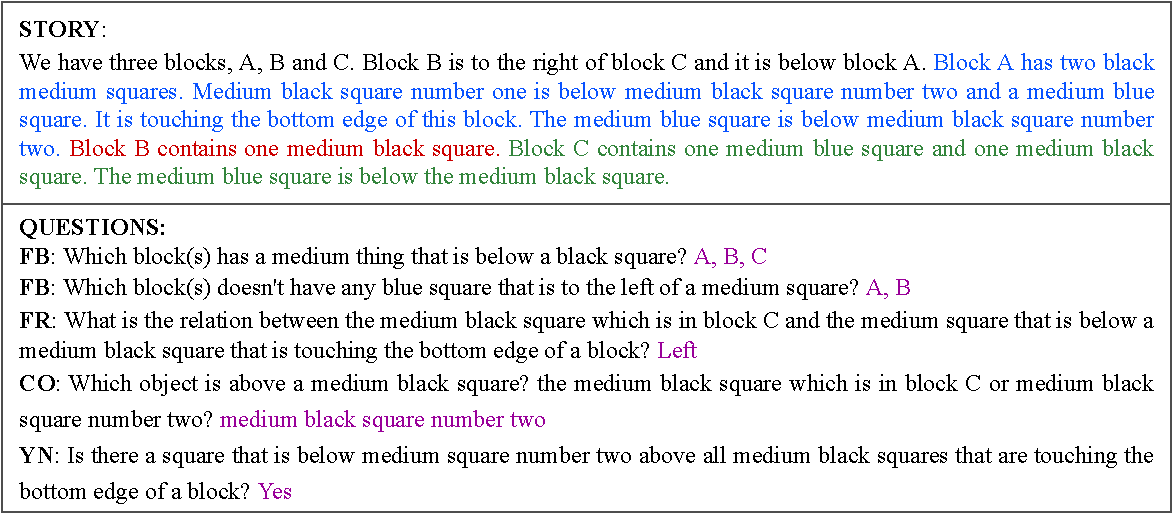
\includegraphics[width=\linewidth]{images/datasets/spartqa_story_sample.pdf}
		\caption{An example story and corresponding questions and answers.
		}
		\label{fig:spartqa_story_sample}
	\end{subfigure}
%	\hfill
	\begin{subfigure}[b]{\linewidth}
			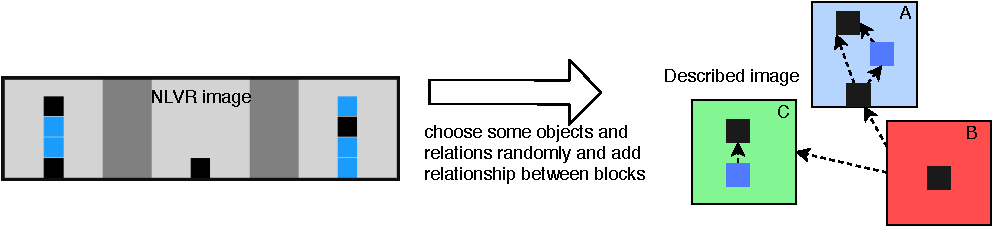
\includegraphics[width=\linewidth]{images/datasets/spartqa_nlvr.pdf}
			\caption{An example NLVR image and the scene created in \cref{fig:spartqa_story_sample}, where the blocks in the NLVR image are rearranged.
			}
			\label{fig:spartqa_nlvr}
    \end{subfigure}
 	\caption{Example from \textsc{SpartQA}. We can see an automatically generated story and corresponding questions and answers.}
	\label{fig:spartqa_examples}
\end{figure}

A very recent work proposes a method called \textbf{Pseudo-Q} to \textbf{automatically create synthetic datasets} that can be used to train visually grounded models \cite{jiang2022pseudo}. Their method consists of leveraging an off-the-shelf object detector to identify visual objects from unlabeled images, and then creating language queries for these objects that are obtained in an unsupervised fashion with a pseudo-query generation module.

The major drawback of synthetic datasets is that they do not always accurately reflect the challenges of reasoning in the real world. Some aspects that are very important in the real world are not taken into account in synthetic images. For example, the orientations of objects, their context and the viewpoint can affect their spatial relation.

\subsection{Natural Visual Reasoning Datasets} \label{sec:natural_visual_reasoning_datasets}

Many vision-language datasets with natural images also contain spatial relations. For example, NLVR2 \cite{suhr2018corpus}, MS COCO \cite{lin2014microsoft}, and VQA \cite{antol2015vqa}.

\textbf{NLVR2} is a dataset for joint reasoning about natural language and images, with a focus on semantic diversity, compositionality, and visual reasoning challenges \cite{suhr2018corpus}. There are 9 prevalent linguistic challenges in NLVR2 among which are spatial relations.
The examples in \cref{fig:nlvr2_examples} require addressing challenging semantic phenomena.

\begin{figure}[ht]
  \centering
    \centering
    \begin{subfigure}[b]{0.49\linewidth}
    \centering
    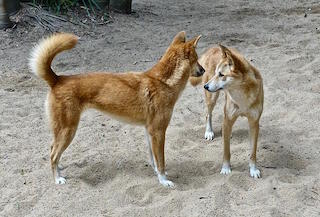
\includegraphics[width=0.49\linewidth]{images/datasets/nlvr2_ex_0_img_0.jpg}
    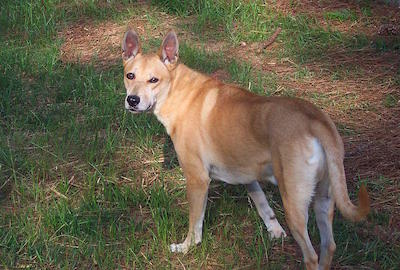
\includegraphics[width=0.49\linewidth]{images/datasets/nlvr2_ex_0_img_1.jpg}
    \caption{The left image contains twice the number of dogs as the right image, and at least two dogs in total are standing.}
     \end{subfigure}
     \hfill
     \begin{subfigure}[b]{0.49\linewidth}
     \centering
    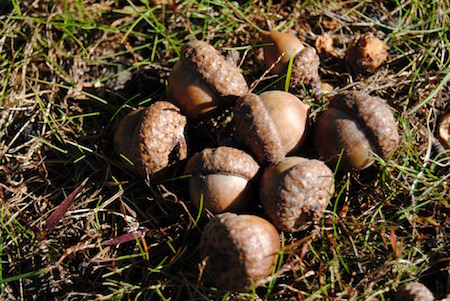
\includegraphics[width=0.49\linewidth]{images/datasets/nlvr2_ex_1_img_0.jpg}
    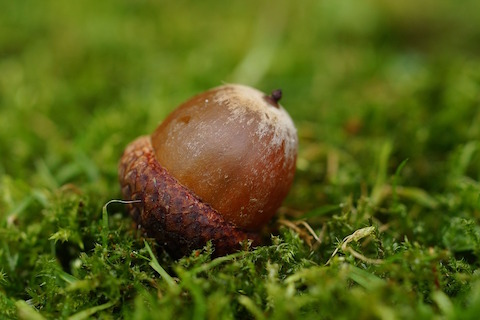
\includegraphics[width=0.49\linewidth]{images/datasets/nlvr2_ex_1_img_1.jpg}
    \caption{One image shows exactly two brown acorns in back-to-back caps on green foliage.}
     \end{subfigure}
    \caption{Two examples from NLVR2, where each caption is paired with two images. The first caption is True and the second one is False.}
    \label{fig:nlvr2_examples}
\end{figure}

\textbf{VQA} \cite{antol2015vqa} is a popular vision and language task. Given an image and a question about the image, the task is to provide an accurate answer. VQA is commonly used as a benchmark to evaluate VQA systems. Questions are generally open-ended but multiple choices are provided for some questions. Some examples are shown in \cref{fig:vqa_examples}.

\begin{figure}[ht]
    \centering
    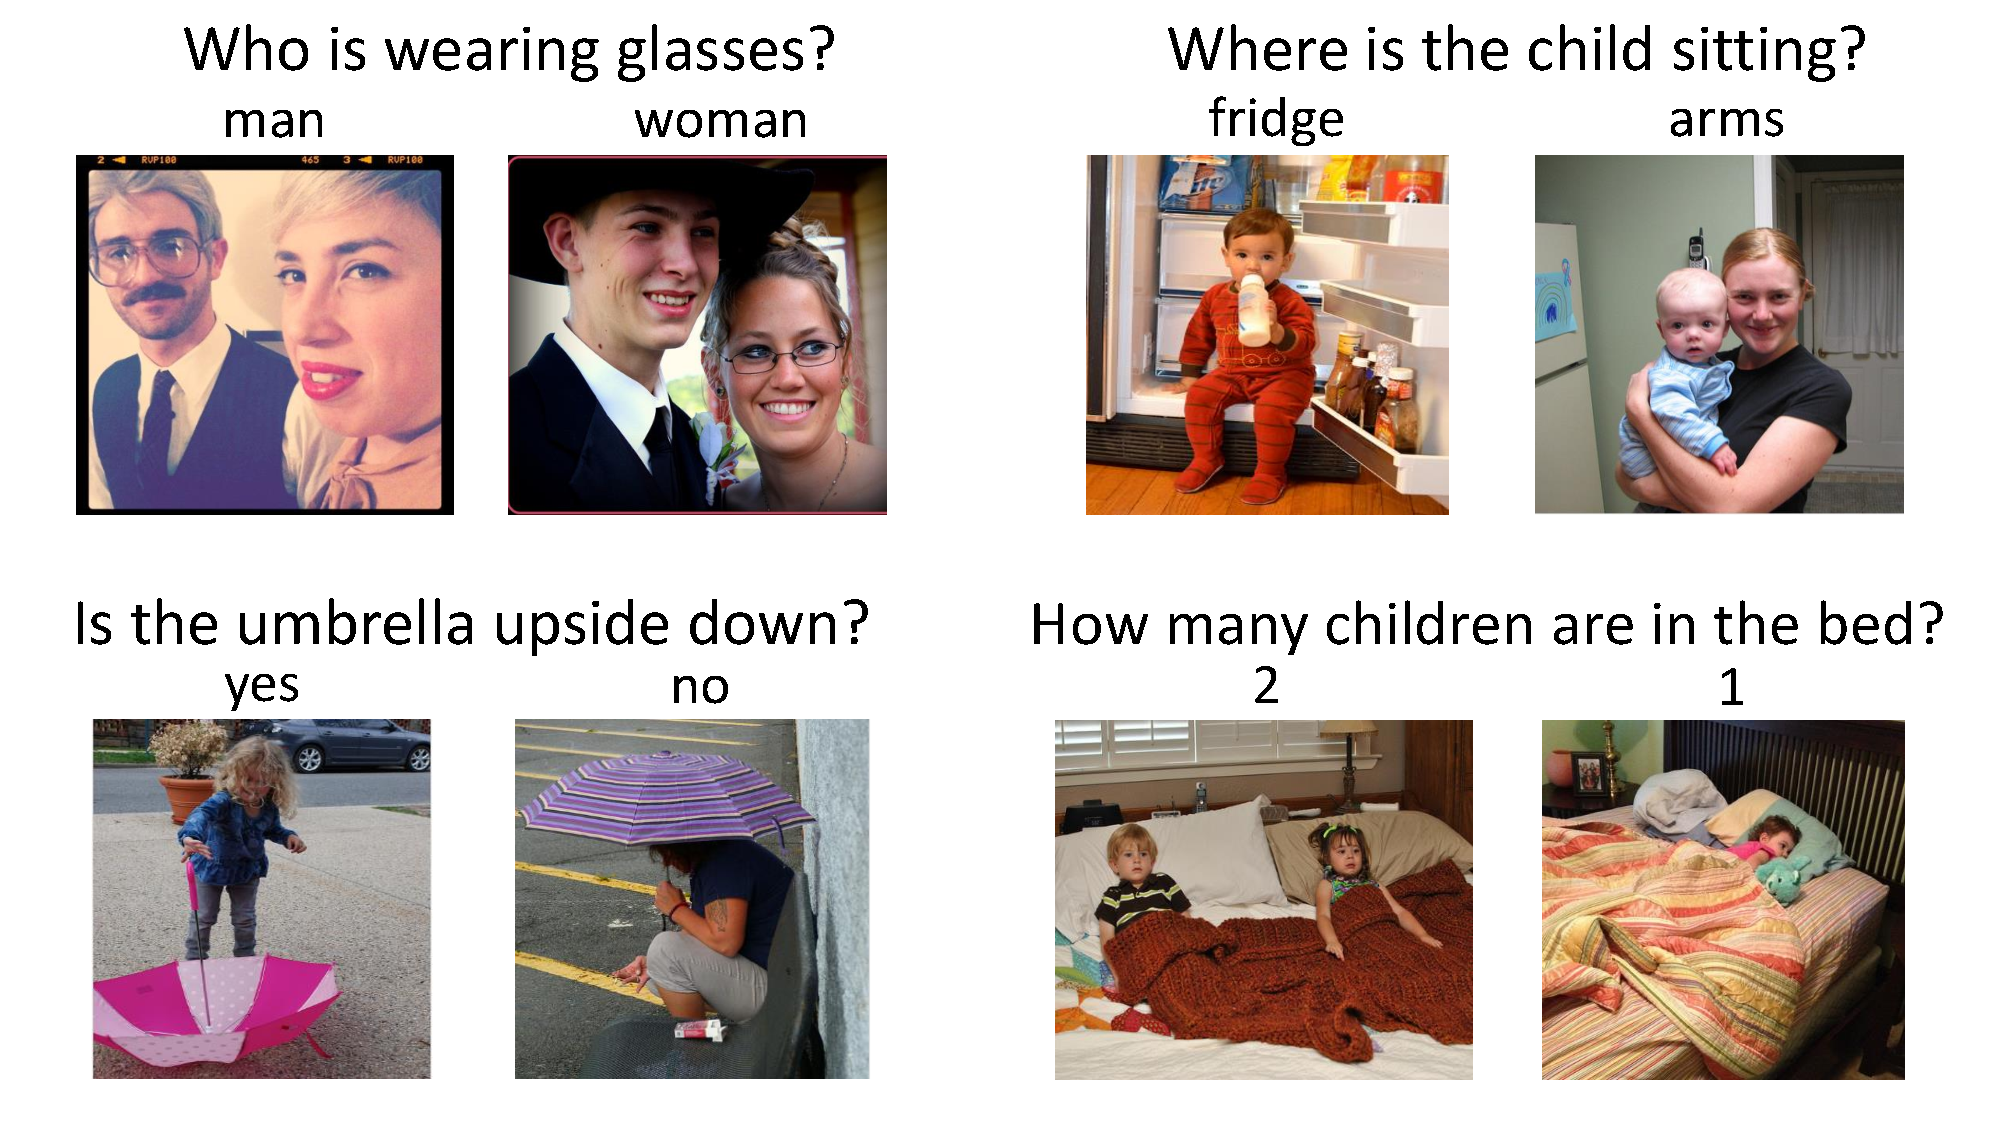
\includegraphics[width=\linewidth]{images/datasets/vqa_examples.pdf}
    \caption{Example images, questions and answers from VQA.}
    \label{fig:vqa_examples}
\end{figure}

The problem with these datasets is that many different challenges are mixed. Sentences have complex lexical and syntactic information. This makes it hard to identify the exact challenges, preventing categorised analysis.

\subsection{Compositional and Spatial Reasoning Datasets} \label{sec:compositional_spatial_reasoning_datasets}

To address the problem of mixed challenges, some datasets focus on a single challenge. For instance, \textbf{Winoground} \cite{thrush2022winoground} focuses on compositional reasoning and \textbf{Visual Spatial Reasoning (VSR)} \cite{liu2022visual} on spatial reasoning. They also contain tags, which enable an in-depth analysis of each visual reasoning challenge. We only provide a short description in this section, but we explain them in detail in the next chapters.

On the one hand, \textbf{Winoground} dataset \cite{thrush2022winoground} is focused on \textbf{evaluating visio-linguistic compositional reasoning} in VLMs. Each instance in the dataset is composed of two images and two captions. Both captions contain a completely identical set of words in a different order. The task is then to match them correctly, which requires the systems to properly deal with composition in natural language. Previous works have shown that language transformers have \textbf{difficulties in learning word order} \cite{sinha2020unnatural,sinha2021matterslittle}. Winoground provides a means to test whether this is also true for multimodal models.

On the other hand, \textbf{Visual Spatial Reasoning (VSR)} \cite{liu2022visual}, whose objective is to test spatial grounding capabilities by covering 65 different spatial relations over natural images collected from COCO \cite{lin2014microsoft}. Given an image, VSR provides a caption which describes a spatial relation between two of the objects that appear in the image. That relation can be real or fake, and that is what the model has to infer. Another advantage of this dataset is that it is annotated by humans. Given its features, we believe VSR is a \textbf{good candidate to evaluate spatial grounding in LMs}.